\documentclass[12p]{article}

\usepackage{geometry} % Requied to change the page size to A4
\geometry{a4paper} % Set the page size to be A4 as opposed to the default US Letter

\usepackage[utf8]{inputenc}
\usepackage{graphicx}
\usepackage{float} % Allows putting an [H] in \begin{figure} to specify the exact location of the figure
\usepackage{wrapfig} % Allows in-line images such as the example fish picture
\usepackage[nopar]{lipsum} % Used for inserting dummy 'Lorem ipsum' text into the template
\usepackage{fancyhdr}
\usepackage[parfill]{parskip} % Makes sure to put line breaks in between paragraphs and have no indentation
\usepackage{dirtytalk} % Used for quotations (\say{quote})
\usepackage[toc,page]{appendix}
\usepackage{caption}
\usepackage{subcaption}
\usepackage{url}
\usepackage{minted} % Used for including code with syntax highlighting: https://www.sharelatex.com/learn/Code_Highlighting_with_minted
\usepackage{fontawesome} % Allows usage of icons within text
\usepackage{enumitem}
\usepackage[final]{pdfpages}
\usepackage{hyperref}
\usepackage{bookmark} % Automatically bookmarks sections in contents section (clickable)

\usepackage[
 style=numeric,
 sorting=none,
 urldate=edtf,
 date=edtf,
 seconds=true
 ]{biblatex}
\addbibresource{references.bib}

\linespread{1.2} % Line spacing
\setlength\parindent{0pt} % Globally suppress indentation
 
\graphicspath{{pics/}} % Specifies the directory where pictures are stored

\pagestyle{fancy} % Use this, if a header on each page with the section title and page number is wanted
\fancyhf{} % Removes all headers and footers, comment this to show page number at the bottom of each page again
\fancyhead[L]{\rightmark} % Sets the section title on the left side of the header
\fancyhead[R]{\thepage} % Sets the page number on the right side of the header

\newcommand{\HRule}{\rule{\linewidth}{0.5mm}} % Defines a new command for horizontal lines
\newcommand{\SlimHRule}{\rule{\linewidth}{0.25mm}} % Defines a new command for horizontal lines

%  A simple AAU report template.
%  2013-03-06 v. 1.0.0
%  Copyright 2010-2013 by Jesper Kjær Nielsen <jkn@es.aau.dk>
%
%  This is free software: you can redistribute it and/or modify
%  it under the terms of the GNU General Public License as published by
%  the Free Software Foundation, either version 3 of the License, or
%  (at your option) any later version.
%
%  This is distributed in the hope that it will be useful,
%  but WITHOUT ANY WARRANTY; without even the implied warranty of
%  MERCHANTABILITY or FITNESS FOR A PARTICULAR PURPOSE.  See the
%  GNU General Public License for more details.
%
%  You can find the GNU General Public License at <http://www.gnu.org/licenses/>.
%
%
%
% see, e.g., http://en.wikibooks.org/wiki/LaTeX/Customizing_LaTeX#New_commands
% for more information on how to create macros

%%%%%%%%%%%%%%%%%%%%%%%%%%%%%%%%%%%%%%%%%%%%%%%%
% Macros for the titlepage
%%%%%%%%%%%%%%%%%%%%%%%%%%%%%%%%%%%%%%%%%%%%%%%%
%Creates the aau titlepage
\newcommand{\aautitlepage}[3]{%
  {
    %set up various length
    \ifx\titlepageleftcolumnwidth\undefined
      \newlength{\titlepageleftcolumnwidth}
      \newlength{\titlepagerightcolumnwidth}
    \fi
    \setlength{\titlepageleftcolumnwidth}{0.5\textwidth-\tabcolsep}
    \setlength{\titlepagerightcolumnwidth}{\textwidth-2\tabcolsep-\titlepageleftcolumnwidth}
    %create title page
    \thispagestyle{empty}
    \noindent%
    \begin{tabular}{@{}ll@{}}
      \parbox{\titlepageleftcolumnwidth}{
        \iflanguage{danish}{%
          \includegraphics[width=\titlepageleftcolumnwidth]{pics/aau_logo_da}
        }{%
          
\includegraphics[width=\titlepageleftcolumnwidth]{pics/aau_logo_en}
        }
      } &
      \parbox{\titlepagerightcolumnwidth}{\raggedleft\sf\small
        #2
      }\bigskip\\
       #1 &
      \parbox[t]{\titlepagerightcolumnwidth}{%
      \textbf{Abstract:}\bigskip\par
        \fbox{\parbox{\titlepagerightcolumnwidth-2\fboxsep-2\fboxrule}{%
          #3
        }}
      }\\
    \end{tabular}
    \vfill
    \iflanguage{danish}{%
      \noindent{\footnotesize\emph{Rapportens indhold er frit tilgængeligt, men offentliggørelse (med kildeangivelse) må kun ske efter aftale med forfatterne.}}
    }{%
      \noindent{\footnotesize\emph{The content of this report is freely available, but publication (with reference) may only be pursued due to agreement with the author.}}
    }
    \clearpage
  }
}

%Create english project info
\newcommand{\englishprojectinfo}[8]{%
  \parbox[t]{\titlepageleftcolumnwidth}{
    \textbf{Title:}\\ #1\bigskip\par
    \textbf{Theme:}\\ #2\bigskip\par
    \textbf{Project Period:}\\ #3\bigskip\par
    \textbf{Project Group:}\\ #4\bigskip\par
    \textbf{Participant(s):}\\ #5\bigskip\par
    \textbf{Supervisor(s):}\\ #6\bigskip\par
    %\textbf{Copies:} #7\bigskip\par
    \textbf{Page Numbers:} ?\bigskip\par
    \textbf{Date of Completion:}\\ #8
  }
}

%Create danish project info
\newcommand{\danishprojectinfo}[8]{%
  \parbox[t]{\titlepageleftcolumnwidth}{
    \textbf{Titel:}\\ #1\bigskip\par
    \textbf{Tema:}\\ #2\bigskip\par
    \textbf{Projektperiode:}\\ #3\bigskip\par
    \textbf{Projektgruppe:}\\ #4\bigskip\par
    \textbf{Deltager(e):}\\ #5\bigskip\par
    \textbf{Vejleder(e):}\\ #6\bigskip\par
    %\textbf{Oplagstal:} #7\bigskip\par
    \textbf{Sidetal:} ?\bigskip\par
    \textbf{Afleveringsdato:}\\ #8
  }
}

%----------------------------------------------------------------------------------------

\begin{document}

%----------------------------------------------------------------------------------------
%	TITLE PAGE
%----------------------------------------------------------------------------------------

\begin{titlepage}
\aautitlepage{%
  \englishprojectinfo{
    Cartographer %title
  }{%
    Project report %theme
  }{%
    Spring Semester 2018 %project period
  }{%
    4 % project group
  }{%
    %list of group members
    Ludvig Alexander Brüchmann (20174692)\\ 
    Johannes Mols (20174921)\\
    Agata Surmacz (20173800)\\
    Ricardo Yaben (20174921) \\
    Boris Yordanov (20174447)\\
    Benas Zauka (20173806)
  }{%
    %list of supervisors
    Jannick Kirk Sørensen\\
    Sokol Kosta
  }{%
    1 % number of printed copies
  }{%
    \today % date of completion
  }%
}{%department and address
  \textbf{Center for Communication, Media and Information Technologies}\\
  A.C. Meyers Vænge 15\\
  DK - 2450 København SV\\
  http://www.cmi.aau.dk/
}{% the abstract
  This report focuses on Google's "Timeline" feature, which tracks user's location periodically. The goal of the project is to inform users about the amount and specifics of the data that is being collected.
  
  This is done with an Android application that is capable of analysing the user's personal location history, which can be explored in several ways. This not only educates the user about their data, but also enriches its value, for their own personal use.
}
\end{titlepage}

%----------------------------------------------------------------------------------------
%	TABLE OF CONTENTS
%----------------------------------------------------------------------------------------

\tableofcontents % Include a table of contents
\thispagestyle{plain} %Sets the page style for this specific page to plain, to remove the header and show the page number at the bottom

\newpage % Begins the report on a new page instead of on the same page as the table of contents 

%----------------------------------------------------------------------------------------
%	INTRODUCTION
%----------------------------------------------------------------------------------------

\section{Introduction}

\subsection{Problem introduction} \label{ProblemIntroduction}

This project specifically focuses on Google and their Google Maps service. With Android having a market share of 75\% in 2017, according to IDC \cite{SmartphoneOSMarketShare}, and Google Maps being pre-installed on every Android device, Google can collect location-based information on a big portion of humanity. In fact, more than 2 billion persons \cite{AndroidMonthlyActiveUsers}, as Google announced in 2017.

As an attempt to give users access to their own data, Google launched "Latitude" in 2009 \cite{GoogleLatitude}. This was a web and mobile app, that tracked your location and shared it with your contacts. This project was retired in 2013. Snapchat, yet another major social media player, released a similar feature on their platform in 2017 \cite{SnapchatMap}. Both of those projects raised a lot of concern about user privacy.

In 2015, Google announced a comeback of the location history \cite{TimelineAnnouncement} (see Figure \ref{fig:timeline}). However, this feature keeps the user's data private and only visible to the user itself. This time line tracks a users movement at all times, and can even determine which kind of transportation he or she used. The user can then view their time line for each day.

\begin{figure}[ht]
    \center
    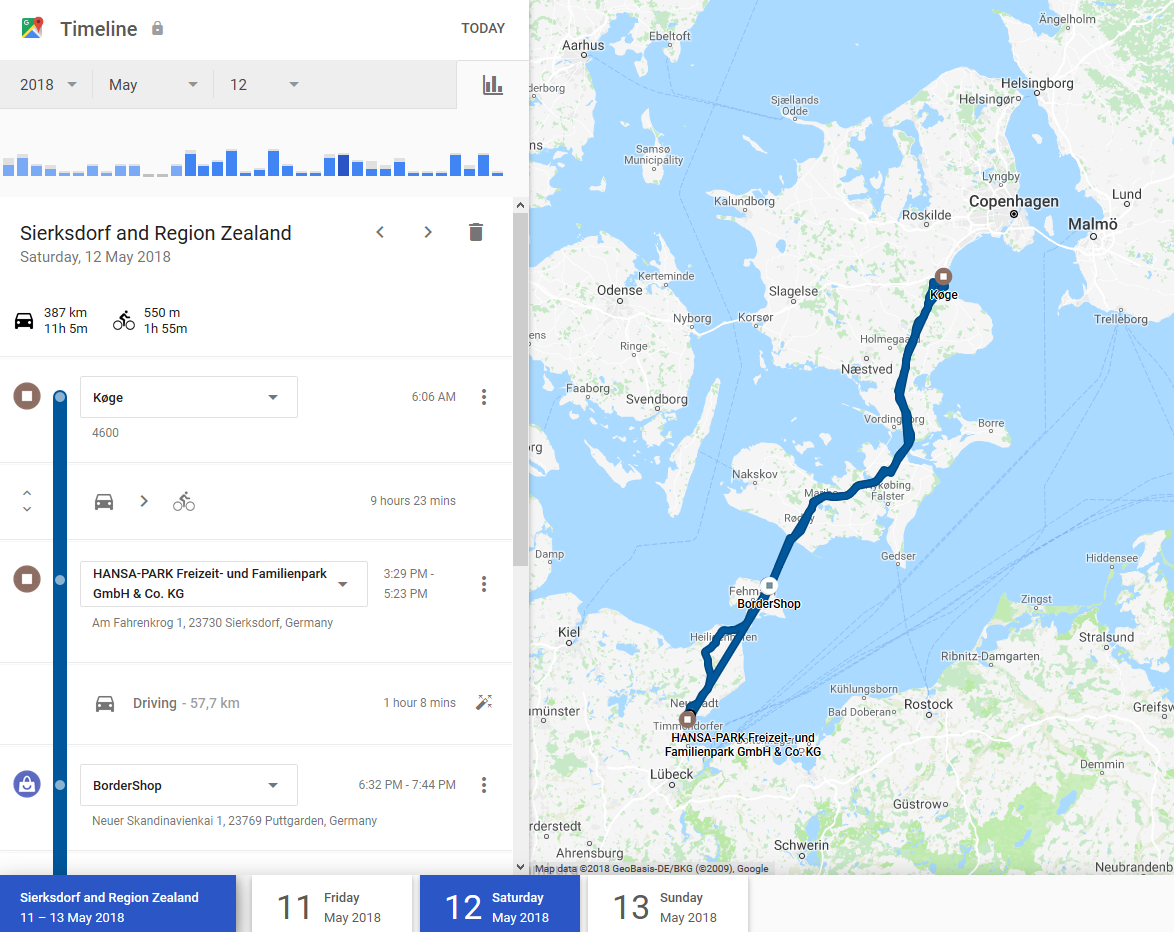
\includegraphics[width=0.85\textwidth]{timeline}
    \caption{Google Timeline}
    \label{fig:timeline}
\end{figure}

Unfortunately, the time line only shows a single day at once and doesn't deliver in-depth statistics or other useful information. And this is where this project kicks in. 

Google lets users download their raw location history as a file, containing bare coordinates, time stamps and presumed activities (like riding a bike, taking the train, etc.). The application behind this project focuses on analysing this data and giving the user an overview of what is being tracked and what the data says about them.

\subsection{Problem formulation} \label{ProblemFormulation}

What information can you extract from the data Google is collecting about you, specifically the location history? How can we use that data for the user’s benefit? Would users be interested in getting advice/tips deduced from their data?

\subsection{Project delimitation} \label{ProjectDelimitations}

This report will not go into market or business analysis of any kind since this project is supposed to be a free and open-source tool to analyse user data. We are not considering to start a business based on this, nor to monetise the app in any way.

Furthermore, privacy won't be part of this report either, as this is a big topic especially with the new \textit{General Data Protection Regulation} in EU law \cite{GDPR}, and will be addressed in the fifth semester of ITCOM. However, we will still address privacy matters regarding the data that is being collected by Google, since this is the foundation of this project.

\subsection{Project introduction} \label{ProjectIntroduction}

Due to increasing advantages brought upon by active developments in various technology, the world has gained a new level of mobility. This was made possible by the steady process of globalisation. As such, technology plays a key role in today's society. Using such technology, both the developers and the users are able to collect, maintain and access sensitive information and data, stored about the user within personal technology, which includes information such as whereabouts (visited locations, areas of visit within a specific time of day/date, etc.), interests, etc. An existing practice of abusing such information is especially predominant online, and used in unison with ads.

Google collects your personal data in order to target ads, as well as to improve your experience when using a specific device. Here are some of the things Google most likely knows about you, if you use your device frequently \cite{GooglePrivacyPolicy}:

\begin{itemize}
	\item Your name, gender and birth date
	\item Your personal cellphone number(-s)
	\item Your contacts list
	\item Your recent Google searches
	\item Websites that you have visited
	\item Where you have been, if you have a phone with Google Maps
	\item Your interests based on searches
	\item Where you work and your home address
\end{itemize}

And these are just a few things, there are many more to name.

However, the way to access this information is not equally as easy for the developers and the users. As such, as our project, we decided to create an application that grants you visual access to the information Google receives and stores for you, and use it for personal benefit. To be more precise, we want to take the information that Google stores about your past and present locations, and make it easily accessible via heat maps, graphs, and diagrams: we want to create a valuable addition to Google's Timeline page because we believe that it has a lot of unused potential with the bast amount of data it has. Furthermore, we want to bring attention to the fact that the access to such information is not limited to just the developers.

%----------------------------------------------------------------------------------------
%	METHODOLOGY
%----------------------------------------------------------------------------------------

\clearpage
\section{Methodology} \label{Methodology}

% The methodology section is supposed to show which methods you used in the project (duh). That means we must explain how we made our app and did our research, not why (but we can reference other sections in the report where we reason for why). So that someone else could in theory replicate our results and app based on our methodology section. I think the P2grp8.pdf file is a good example of a methodology section. Also it is important to include fancy methodological words like: quantitative, qualitative. It is good to say in order to achieve goal A we needed to do task B, but don't explain in too much detail why A or B are necessary, save that for the "real" part of the report. It is also good to end sections with something like, by using some method we were able to complete task B and accomplish goal A, and argument for the method itself.

    \subsection{Idea specification}
	
	This project needed to fulfil the requirements specified by the semester theme to create an Android application. To come up with an idea for our app we started brainstorming and wrote all of our ideas on a whiteboard. To come up with an idea we discussed various technologies we had experiences with. After narrowing down our list of ideas we looked into which ideas best fit the scope of our project. We wanted to make something new and innovative, so it was important for us that our idea for an app didn't already exist, or at least provided something new to the user other apps didn't already. With this in mind we were able to further narrow our list of ideas. In order to pick a final idea we looked at a more societal context, and with the recent focus on privacy and protection of personal data we decided to make an app visualising the location data Google stores about their users.
	
	\subsection{State of the Art}
	
    The State of the Art is an important tool we used to analyse and highlight good, patented solutions for different areas of functionality applied in the project or research material in question. We did so by looking at other apps and services that provide a similar service to our idea. We looked at other services and apps that implement the use of Google's tracking services, and seeing whether we could find something that we could use to further benefit our system.
	
	When beginning research, we first decided to shift our focus towards scientific material: publications and articles on Google's tracking services. Said material included the intricacies of security and user-privacy when handling such information, which, while not too important to us in terms of implementation for this project in particular, were still critical to understand. More significant to us were details on how various services process location-based information, and what can we do with said information. In addition, we needed a deeper understanding of exactly what information Google records, and how it stores it. We have found two research papers: one on IEEE website (The world's largest technical professional organisation for the advancement of technology) and one Google's research lab paper. In such regards, this researches were incredibly beneficial.
	
	Afterwards, we looked at potential existing solutions, and picked out a couple that provided interesting services, which we would be able to try out and make a few comments on, weight their benefits and drawbacks and decide whether to provide such services ourselves, as well as whether it was possible to improve upon said services when developing our software.
	
	We will be discussing the fruits of our labour in section \ref{sec:StateOfTheArt}.
	
	\subsection{Requirements}
	
	\subsubsection{Analysis Techniques}
	
	Analysing a project(–s) before implementation is essential for both development and management. Such analysis is used extensively to find requirements, inspirations, as well as specify various ideas. These insights can be used to determine the amount and variety of resources required for the project to be successfully launched.
	
	We've split up our analysis into sections for state of the art, which we relied upon to find inspirations, and storyboards, which were used for the specification of requirements.
	
	\subsubsection{MoSCoW Prioritisation}
	
	For the project, we used the MoSCoW model due to time constraints. The MoSCoW method separates tasks into four categories to clarify priorities during the development stage:

    \begin{itemize}
        \item Must have
        \item Should have
        \item Could have
        \item Won't have
    \end{itemize}
    
    Using research from the state of the art, we were easily able to define and identify what basic functionality our app must have to be functional. We then further discussed what other functionalities we would like our app to have, based on our brainstorming sessions.
    
    From all of this, we organised the features and requirements into the four MoSCoW categories to guide us in the development stage. The MoSCoW method is very useful when working collaboratively, since it helps prioritise the work effort and maintain focus on producing a functional product.
	
	\subsubsection{Storyboard}

	Storyboarding is an important tool in software development, used to identify specifications for a software. It is applied as visualisation of different scenarios that illustrate the important steps of the user experience. Said storyboard is then modified, based on specific individual needs of both the user and the manufacturer. The method of storyboarding is important because it is fast and cheap to produce, and it helps to finalise abstract ideas. In addition, said method is also beneficial to the user, providing a clear, visual depiction of how the software is supposed to function, and is going to work. Using storyboards to create software gives the developer a realistic view on said software. With that in mind, the primary benefit of using storyboards is for the developers to understand user experience, which is used to gather requirements for software, and that is why we chose to apply the use of storyboards for this project.

	We used the \textit{Storyboard That} \cite{StoryboardThat} online services to design our storyboards.
	
	\begin{figure}[ht]
	    \center
        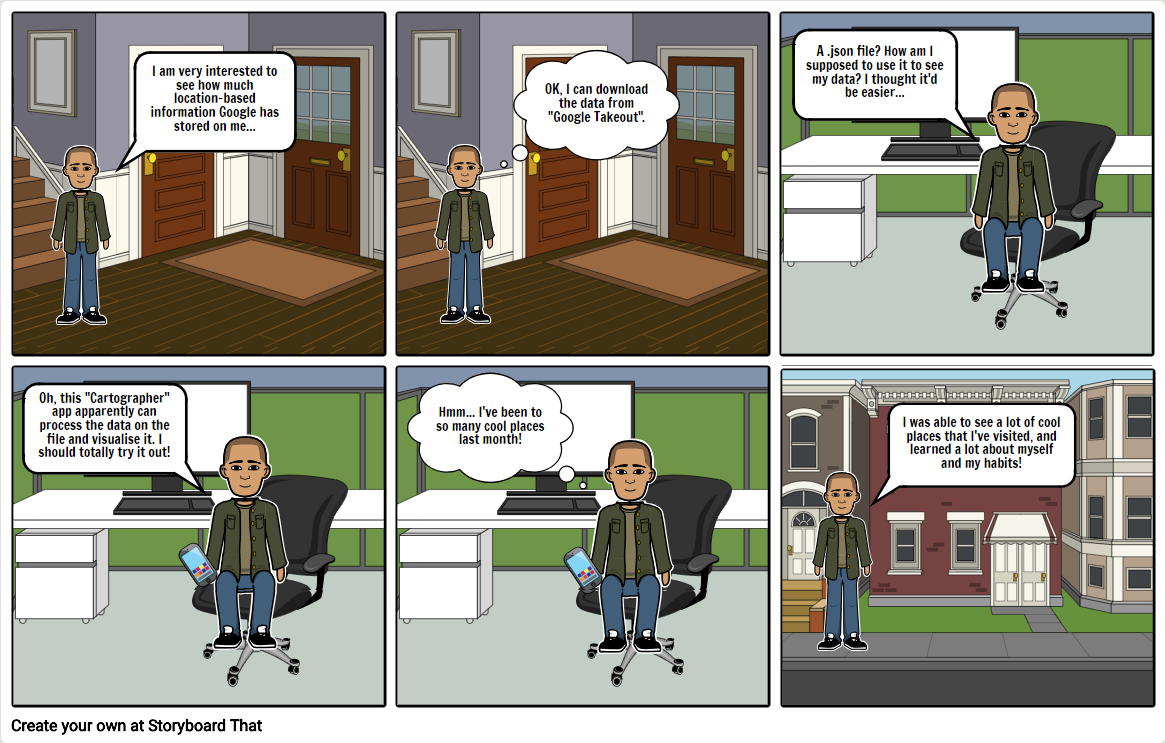
\includegraphics[height=8cm,keepaspectratio]{pics/story1.png}
        \caption{Storyboard 1}
    \end{figure}
	
	The purpose of the first storyboard is to visualise how location-based data can be accessed in a household-esque scenario. The outline of the storyboard involves a young man, showing interest in the data received and stored on him by Google. He heads to "Google Takeout" in hopes of downloading said information, but has little knowledge regarding the treatment of the file he receives. Not knowing how to access the stored data, the man turns to "Cartographer" to convert the file into visual information.
	
	From these pictures, we can see that a major requirement is data visualisation.
	
	\begin{figure}[ht]
	    \center
        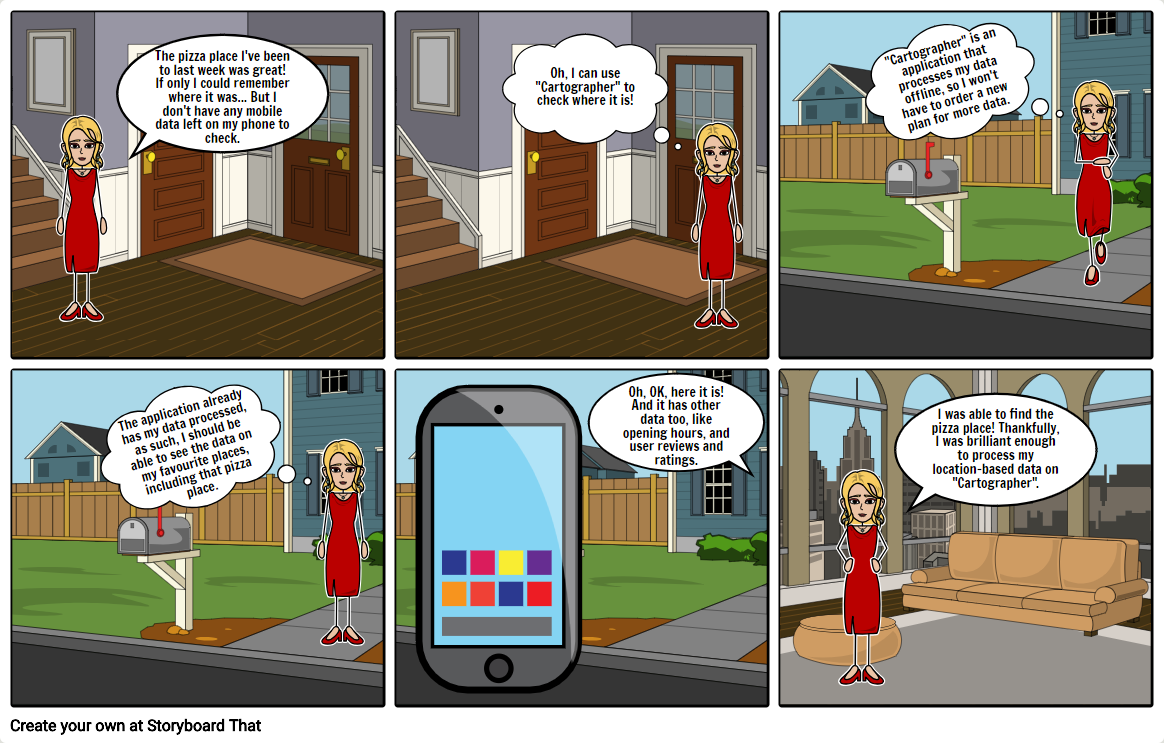
\includegraphics[height=8cm,keepaspectratio]{pics/story2.png}
        \caption{Storyboard 2}
    \end{figure}
	
	The purpose of the second storyboard is to visualise how location-based data can be accessed on the go, without requiring the use of Wi-Fi or other forms of internet access. The outline of the storyboard involves a woman who forgets the location of a place she'd visited prior, and does not have sufficient mobile data to look up said location on her phone. Luckily for her, she remembers that she had used "Cartographer" and has the data relating to that location on the application. As "Cartographer" does not require internet access to process data, the woman is able to access the information she requires, as well as other information Google has on that location, and she is able to make it to her desired destination.
	
	From these pictures, we can deduce that user requirements also include the ability to visualise data without direct access to the internet, as well as access information stored on various locations directly from Google.
	
	\subsection{Process Model (Waterfall)}
	
	%\cite{WaterfallArticle}
	
	The Waterfall software development model is a plan-driven process model that was first formally described by Winston W. Royce in 1970 \cite{Royce1970}. It consists of five basic steps that can be seen in Figure \ref{fig:WaterfallDiagram}.
    
    \begin{figure}[ht]
        \center
        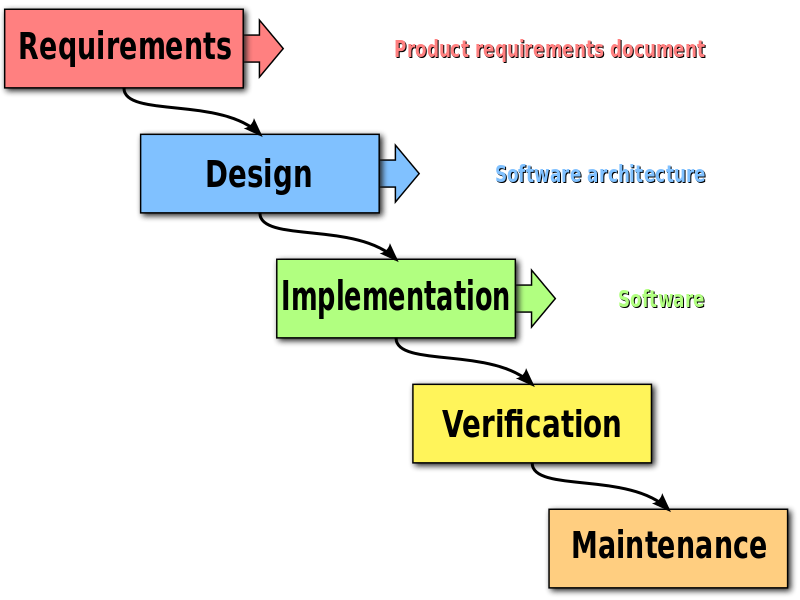
\includegraphics[width=0.75\textwidth]{methodology/800px-Waterfall_model.png}
        \caption{Waterfall model \cite{WaterfallDiagram}}
        \label{fig:WaterfallDiagram}
    \end{figure}
    
    This process model is very popular and widely used in many engineering and software development projects. It consists of several steps that build on top of each other, with the requirement that no other task can be started before the previous task is finished. It is a rigid approach to a task and previous work can hardly be changed after completing any of the given steps.
    
    Because of this rigid design of the Waterfall model, it has its fair share of critique, and for good reason. Clients may change their requirements mid-development and a revision is not possible or highly expensive. Many failed projects blame the Waterfall model for its fixed steps.
    
    Nevertheless, it is still an effective and, most importantly, simple process model for many projects. If a project has very well defined requirements that are not subject to change, it most likely makes sense to use a plan-driven model over an agile one.
    
    We will explain why we chose the Waterfall model in section \ref{sec:ProcessModel}.
	
	\subsection{Application Design}
	Project visualisation is very important in that it creates the foundation for the entire process flow. Without a sketch, or a draft, working on a single application in a group of individuals would be almost impossible, as everyone has different ideas of how a good application has to look and function. The right visualisation is crucial for follow-up decisions, the application’s structure and data analysis. For that reason, to ensure that all of us had mutual intentions and goals when it comes to the structure of this application, we decided to create desirable mock-up visuals for our application using the online services of the “Marvelapp” sketching app. In addition, as we wanted the application to be accessible to a broader scale of users, not just ones exclusively limited to mobile phones, despite them being the major demographic, we decided to develop the visualisation with tablet users in mind as well.
	
	\subsection{Implementation}
	%Finding the right APIs%
	%Authentication%
	
	When it came to implementing our idea we refereed to our MoSCoW prioritisation and split up the different tasks amongst the group. To structure the tasks ahead we used a Kanban board and ordered the tasks according to our MoSCoW prioritization. We used ZenHub\cite{Zenhub} as our Kanban board since it provides direct GitHub integration, using those two combined helped visualise our progress and keep everyone up to date.
	
	Using a Kanban board can enhance the workflow when working collaboratively, it shows tasks and splits them into categories showing the status of the task. It proves useful once a member finishes a task since they can quickly see what other members are working on and pick their next task accordingly. 
	
	
	\subsection{User Research}
	It is highly important to make sure that an idea for an application is actually in demand by enough possible users. User research gives an insight into this demand, and can also bring important feedback on certain features, the application design, availability, price and more.
    
    In this case, we constructed an online survey/questionnaire \cite{Survey} with the Google Forms \cite{GoogleForms} service. The goal of this survey is to test participants on their awareness of location-related data collection, in particular by Google. The survey asks questions like \textit{"Do you believe your phone tracks your location?"} and follows up with questions about whether participants think that data is accessible to them and if they have ever seen it.
    
    The second part of the survey focuses on the participant's willingness to use our application, by asking them how comfortable they are with sharing their location history with our this third-party service, and what features they would like to see. The participants also get an option to not use our application, which is followed up by asking them what the reason for that is (e.g. privacy concerns, lack of interest, ...).
    
    For surveys to be meaningful, it is not only important to get many answers, but also to get diverse answers from different persons with different backgrounds. For this to work, the survey has to be shared on different platforms.
    
    The first and easiest way to distribute the survey is to post it on Facebook, in an AAU group made for this specific purpose. Furthermore, we distributed the survey on various different platforms (e.g. Surveycircle \cite{Surveycircle} and Poll Pool \cite{PollPool}).

%----------------------------------------------------------------------------------------
%	STATE OF THE ART
%----------------------------------------------------------------------------------------
	
\newpage
\section{State of the Art} \label{sec:StateOfTheArt}
	\subsection{Introduction}
	
Before we started to invest our time intended for this project we went through scientific publications, articles and Google documents to make sure this project is worth it. We have also looked for similar applications and solutions to find out about existing solutions. The results of our research are described below. 

To further progress the development of the application, it is essential to understand Google and its ways of collecting and processing information. As such, first and foremost, we’re going to look at Google’s policies regarding user information tracking.

Google collects information in the following ways\cite{GooglePrivacyPolicy}:

\begin{itemize}
    \item When you sign-up for a Google account, you are required to share your personal information. That includes your name, email, tel. number, credit card, etc.
    \item Collecting information through the use of services. This includes device-specific information (such as operating system, hardware model, etc.), log information (search queries, tel. log info., tec.), local storage, as well as location information (personal location, IP address, GPS, etc.), among other things.
\end{itemize}

\subsection{Existing solutions}
The central focus for us is the collection of information that is related to your device's location. As mentioned beforehand, this can be done through things such as the IP address, GPS, as well as Wi-Fi access points and even cell towers that your phone is connected to. Accessing that information is quite tricky for the user, however, because Google is not fully transparent about the available options to acquire that data. Additionally, there are people who use Google's services without realising that they're sharing said information with the provider.

With that being said, we were able to identify several applications that allow the user base to access the location-based information that Google has stored, and visualise the data without requiring the users to "jump through hoops" to initiate the process (i.e. the application keeps the whole process as simple and efficient as possible, complete with guides and directions for the user to follow).

\subsubsection{Google Timeline}

The "Google Timeline" is a functionality of Google Maps that helps you find the information on the places you've been to, as well as the routes you frequently travel by. It also allows you to view said information by date, mode of transport or type of activity.

Pros:
\begin{itemize}
    \item The timeline is private, and separate for each individual account
    \item The timeline itself uses the language you've selected in your user preferences
\end{itemize}

Cons:
\begin{itemize}
    \item It only shows you specific information that you've collected throughout the past 24 hours
\end{itemize}

\begin{figure}[ht]
	    \center
        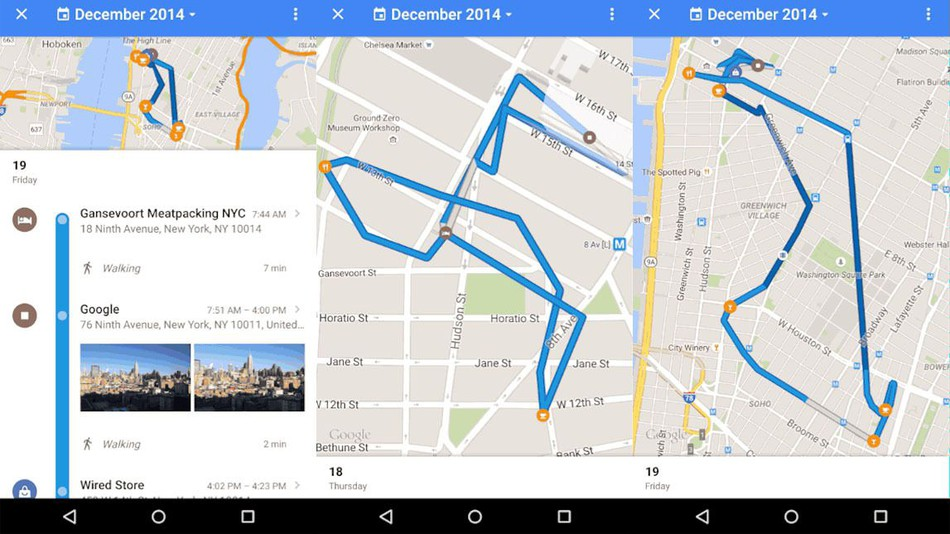
\includegraphics[height=8cm,keepaspectratio]{pics/state-of-the-art/Google_Timeline.jpg}
        \caption{Google Timeline}
    \end{figure}

\subsubsection{locationhistoryvisualizer.com}
It is a website that processes raw Google Location History, and converts it into an interactive map, using an open street map to locate pins via satellite view. The user can view each individual location recorded, as well as see accurate information on each visited location. The user can also search for different locations, based on individual address, name, or even latitude and longitude, and filer each location by accuracy, distance travelled, time, and more. In addition, the user can highlight gaps in the data so that they’d be marked for further analysis, as well as view the compressed data on any Android or iOS device, as well as any Windows, Mac, or Linux computer. The application also features quite a bit of customisation, allowing full freedom regarding how you want your information to be showcased.

Pros:
\begin{itemize}
    \item Convenient, online web-based application
    \item The info that is provided on the website is particularly broad
    \item The website offers free trials, upon request
\end{itemize}

Cons:
\begin{itemize}
    \item Expensive, price is not approachable by every-day users.  Some additional features are also locked behind a Premium-only (“Enterprise”) feature
    \item No side-functionality makes the application particularly specific.
\end{itemize}

\begin{figure}[ht]
	    \center
        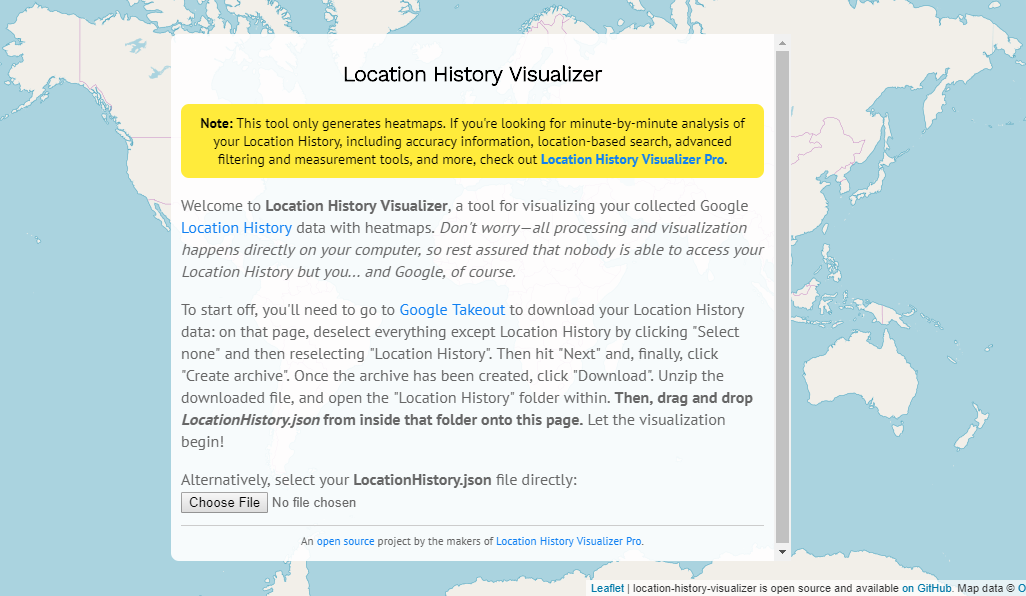
\includegraphics[height=8cm,keepaspectratio]{pics/state-of-the-art/lochistory.png}
        \caption{locationhistoryvisualizer.com}
    \end{figure}

\subsubsection{theyhaveyour.info}
It’s a website that allows you to upload a personal .json file from “Google Takeout” to showcase your location history. It is a rather simple website in terms of design, with all it having is the necessary instructions on how to download your .json file. Once you do upload your location history to the website, however, you are presented with a heat map of your most frequented locations. In addition, the website also contains a list of the top most visited locations (that includes the country, address, and region), a box that cites how many times you’ve been tracked during a certain time duration, as well as a button to switch up the heat map between terrain map, road map and satellite view.

Pros:
\begin{itemize}
    \item Information processing takes place offline, ensuring complete security
\end{itemize}

Cons:
\begin{itemize}
    \item The .json file needs to be manually uploaded
    \item The map itself serves very little in terms of functionality. While it displays the heat map accurately, there is a lack of function regarding the heat map’s settings
\end{itemize}

\begin{figure}[ht]
	    \center
        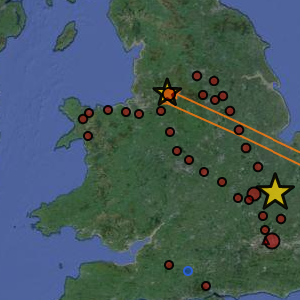
\includegraphics[height=8cm,keepaspectratio]{pics/state-of-the-art/info.png}
        \caption{theyhaveyour.info}
    \end{figure}

\subsubsection[iPhoneTracker - iOS Application]{iPhoneTracker - iOS Application \cite{iPhoneTracker}}
This application generates location history points on the map, based on backup files on the phone. It allows you to generate heat maps using open-source services like the "Openheat" map script. This application is very close to our product vision. It has some system limitations (this application is only available for iOS devices), but we can get from it inspiration about the design of the app as well as the way their heatmaps look like.

Pros:
\begin{itemize}
    \item The presented information is incredibly accurate, and the application itself does not record any data
    \item The application is free to download, meaning there's no excuse not to give it a try
\end{itemize}

Cons:
\begin{itemize}
    \item The application is exclusive to iOS devices
    \item The code is open-sourced, which results in lack of security
\end{itemize}

\begin{figure}[ht]
	    \center
        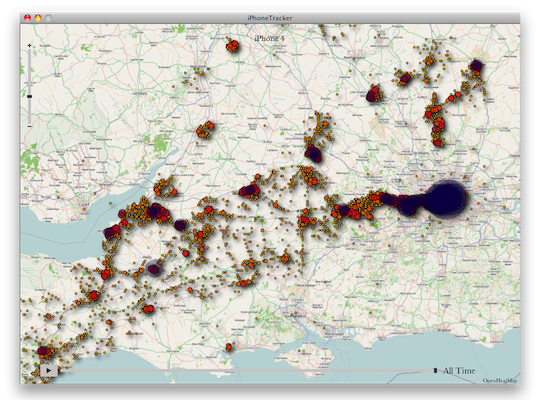
\includegraphics[height=8cm,keepaspectratio]{pics/state-of-the-art/iOS_track.png}
        \caption{iPhoneTracker}
    \end{figure}

\newpage
\subsection{Scientific publications}
\subsubsection["Analysis of User Privacy in Mobile Geo-location sharing"]{"Analysis of User Privacy in Mobile Geo-location sharing" \cite{UserPrivacyPaper}}

This research is mostly about user-privacy, but this part is not the most important for us as our project is not about the security. The reason why we decided to mention it is that it explains how the user's personal data can be gathered when geo-location services are paired with third party domains. It helped us to get an overview regarding if and how we can relate our geo-location points with the places names. The other idea that we get from this research is that even though we should not bother with security it would be good to have at least password protection to prevent unwanted third-person access.

\subsubsection["Extracting Patterns from Location History"]{"Extracting Patterns from Location History" \cite{GoogleLabPaper}}

This is the official Google research lab paper that explains how location-based services work. This paper lets us get an overview of how the geo-points that we require are created and calculated, as well as how many geo-points we can get in a specific time frame. It also explains the accuracy of the geo-points we can get, depending on services, like GPS, Wi-Fi, and cell tower triangulation, being on or off the device. It also shows how to compute frequently visited places (favourite places, in our case), and how the commute analysis works. Thanks to that research we were able to, with the basic knowledge on location history, start to figure out what technical resources we may need for our application.

\newpage

\subsection{Articles}
\subsubsection["How to map your Google location history"]{"How to map your Google location history" \cite{HowToMapArtc}}

This article explains the way Google JSON files are written. It helped us understand the meaning of such files, and the single lines written within them. Due to this research, we are able to know what data we can find: dates, distances and probable activities, based on geo-location. It also inspired us to find out what tasks should and can our application perform.

\subsubsection["If you’re using an Android phone, Google may be tracking every move you make"]{"If you’re using an Android phone, Google may be tracking every move you make" \cite{IfYoureArtc}}

This article provides the general information about the type of data that Google records. We used this article at the beginning of the project to get overall knowledge about geo-points and their relation to activities.

\subsubsection["Google’s Mobile Location History"]{"Google’s Mobile Location History" \cite{GooglesMobileArtc}}

This article is about location history. It serves us as an additional source of information regarding Google's location-based services.

\newpage
\subsection{Conclusion}

To summarise, by reviewing both the strong and weak points of each of those applications, we decided for our application to put our focus into replicating their adaption of the heat maps (with some of our own additional twists), as well as implement the addition of statistical visual data, and have it be filtered by date, to further enrich positive user experience. We've researched scientific publications and various research papers to learn more about an abundance of different details surrounding the services that are able to be provided by applying the use of location-based data that is gathered by Google, as well as to what imaginable extent could we push our ideas to create unique, never-before-seen services.

%----------------------------------------------------------------------------------------
%	PROCESS MODEL
%----------------------------------------------------------------------------------------

\newpage
\section{Process Model (Waterfall)} \label{sec:ProcessModel}

Choosing a process model for our software development was relatively straightforward. Because of the nature of this project, which has well-defined requirements, and didn't expect them to change during the work process, we chose a plan-driven process model, instead of an agile one. We had made requirements on what the application must be able to do, we created sketches of the application. So we knew what features we need to implement and how they should look like.

While considering agile software development practices such as \textit{Scrum} \cite{Scrum}, \textit{Kanban} \cite{Kanban} or \textit{Extreme Programming} \cite{ExtremeProgramming}, we quickly realised that many of the main concepts of agile software development are not applicable to our project. 
We don't need to collaborate with customers, because there are none. As said before, this project primarily focuses on informing users about aspects of data collection and is not supposed to be a business. It is sufficient for us to release a free and open-source application to improve user's awareness and personal benefit of their data. While still listening to user's opinions and wishes, we do not need to adapt to changes in "customers" demands.

Furthermore, we do not believe that short iteration-cycles of agile development are helpful or necessary in our case, because we wanted to focus on building the most important features such as data processing and a few data visualisation features first, instead of changing up the tasks all the time.

While also considering plan-driven software development models, we decided to use the Waterfall model because of it's simple and fixed steps, which we naturally followed when starting the project, before even considering which process model to choose.

We are fully aware of many critics of the Waterfall process model, such as Conrad Weisert \cite{WaterfallSucks}. Among other points, he is stating that the "results are \textit{frozen}" after completing a stage, and it is hard to go back and revise certain aspects. He also states that it is not possible to work on a next stage while the current stage isn't completed, which could lead to wasted time.

After considering the criticism, we still decided to go for it because we believe that we have strong and static requirements as well as a solid idea of the early application design. Also it's simple structure allowed us to spend less time on project management and discussions, which gave us more time for programming.

The Waterfall model consists of the five following steps:
\begin{enumerate}
    \item Requirements
    \item Design
    \item Implementation
    \item Verification
    \item Maintenance
\end{enumerate}

While working on the project, the first step was to gather requirements so we are all on the same page as to what kind of application we will build and what it is supposed to be able to do. This is described in section \ref{sec:Requirements}.

After having all requirements gathered, we ventured out to create sketches of how the application is supposed to look like. This is described in section \ref{sec:SoftwareDesign}.

The third and most exciting part of the waterfall model is the implementation, which we started to do after completing the first two stages with a clear picture of the application in mind. A detailed description of how the implementation was handled can be found in section \ref{sec:Implementation}.

Coming to the fourth step of the process model, the testing, we, unfortunately, didn't get as far as we have hoped. The implementation of all features took a long time and we didn't get to a stage where application was ready for testing, which is why we only did internal testing during the developments process, but we didn't collect input from potential users.

The fifth step, maintenance, can be discarded in our case, because we are not publishing the application on the Google Play Store, nor distribute it in any other way.

%----------------------------------------------------------------------------------------
%	REQUIREMENTS
%----------------------------------------------------------------------------------------

\newpage
\section{Requirements} \label{sec:Requirements}
Requirements are statements on what a system \textit{must} or \textit{should} do. They list limitations on the resources or design, as well as \textit{how well} the system performs. We created the user requirements during our initial brainstorming sessions, but not all of them will be included in the MVP as stated in the Project Delimitation. 

\subsection{User requirements} \label{sec:UserRequirements}
Statements, in a non-technical language of the services the user expects the system to provide, as well as any constraints that might be relevant \cite{Requirements}. For Cartographer we defined the following user requirements:

\begin{itemize}
    \item Must be able to process location history files from Google (in the \texttt{.json} file format)
    \item Must be able to select a date range for shown data
    \item Must be able to visualise the processed data as a heat map
    \item Must be able to visualise the routes they most frequently use as map, with outline routes
    \item Must be able to visualise the places they most frequently visit, as markers on a map
    \item Must store data locally
    \item Must not share data with third parties
    \item Should be able to encrypt all data
    \item Should remind users to delete their downloaded data after processing
    \item Should be able to to visualise the data without an internet connection
    \item Should be able to receive advice on how to improve users lifestyle
\end{itemize}

\subsection{System requirements} \label{sec:SystemRequirements}
System requirements list any operational and hardware constraints that the system needs in order to operate \cite{Requirements}.
\begin{itemize}
    \item Must have Android OS \cite{Android} version 4.4 and higher that is compatible with Google Play\cite{AndroidPlayStore}
    \item Must have an internet connection
    \item Must have 200 MB of available disk space
    \item Must have a Google account
    \item Must have the \textit{Timeline} feature activated in Google Maps
\end{itemize}

%----------------------------------------------------------------------------------------
%	ARCHITECTURAL DESIGN
%----------------------------------------------------------------------------------------
		
\newpage
\section{Software Architecture} \label{sec:SoftwareArchitecture}
    \subsection{Introduction}
    This section describes the structure of our system at a high level. It includes the application's architecture and also how it interacts with external services and users.
    
    \subsection{Context Diagram}
    Context diagrams are behavioural diagrams, that show the system as a single top-level process, along with relationships it has with external entities (users, other systems, data storage, etc) \cite{ContextDiagram}.
    
    \begin{figure}[H]
        \center
        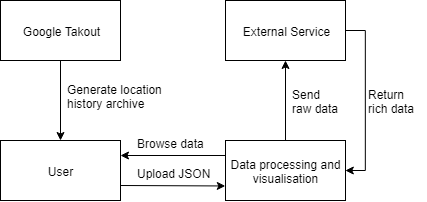
\includegraphics[width=0.8\textwidth,keepaspectratio]{pics/diagrams/ContextDiagram.png}
	    \caption{Context Diagram}
    \end{figure}
    
    At a high level our app acts as a hub, that process and stores the data, that was imported by the user. The application uses external services to aid the analysis of the data, which is visualised afterwards.
    
    \newpage
    \subsection{Use case Diagram}
    A behavioural diagram that describes actions (use cases) that systems perform when they operate, when in use by an actor (user). The elements in the diagram describe what the system does, while omitting information on how it functions \cite{UseCaseDiagram}. 
    
    \begin{figure}[H]
        \center
        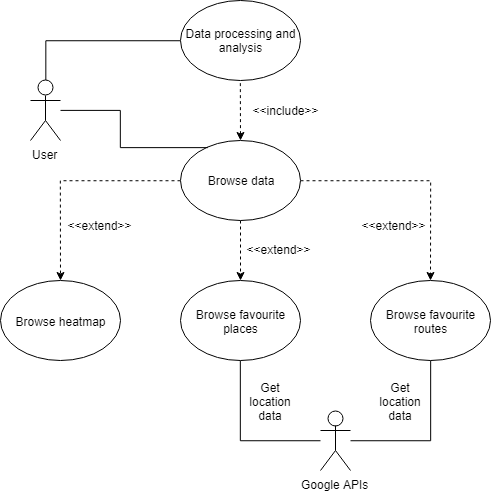
\includegraphics[width=0.8\textwidth,keepaspectratio]{pics/diagrams/UseCaseDiagram.png}
	    \caption{Use Case Diagram}
    \end{figure}

    In our diagram we can see the main actors are the User of the app and the Google APIs. Our system is split into two nodes, which represent its two main functions - data processing and visualisation. The data browsing node can be considered as an inclusion of the data processing node, because that's where the data is stored and queried from. The data browsing is extended by 3 different nodes, which represent the different use cases. Some of them use external APIs to implement the desired functionality.
    
    \newpage
    \subsection{Class Diagram}
    
    Class diagrams give an overview about the architecture of a software, by giving detailed information about field variables, methods, inheritance and more. The following class diagrams are split up to give a better overview without having too many nodes on one diagram.
    
    \begin{figure}[H]
        \center
        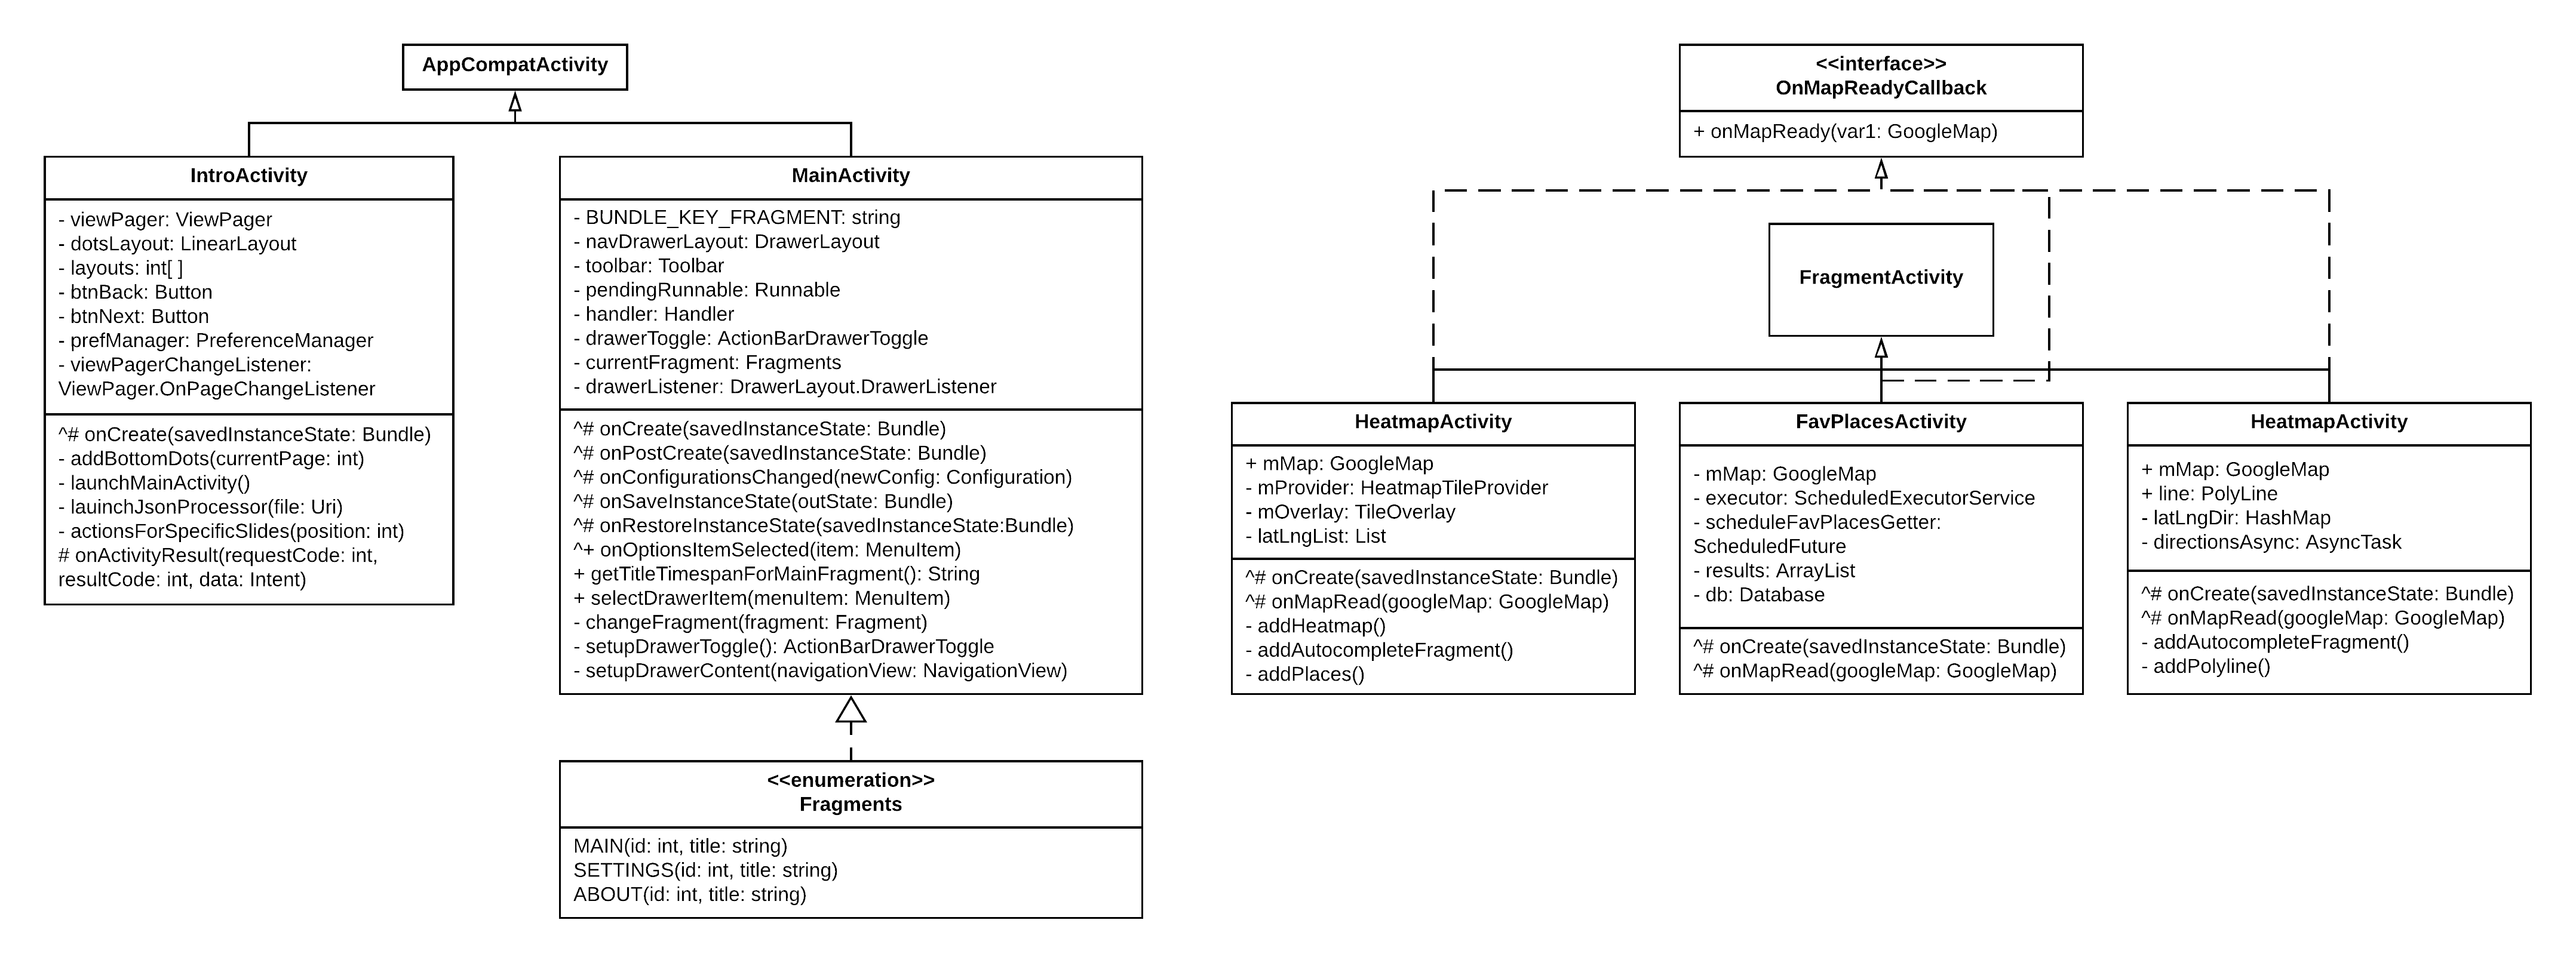
\includegraphics[width=1.0\textwidth]{class_diagram/class_diagram_1}
	    \caption{Class Diagram of Activities}
	    \label{fig:class_diagram_activities}
    \end{figure}
    
    The first class diagram (see Figure \ref{fig:class_diagram_activities}) shows five of the six activities in the application. The first is the \texttt{IntroActivity}, which displays the initial slides to guide the user through uploading his personal location history file. This activity launches the \texttt{MainActivity}, which lets users choose different types of visualisations that will start one of the remaining activities.
    
    \begin{figure}[H]
        \center
        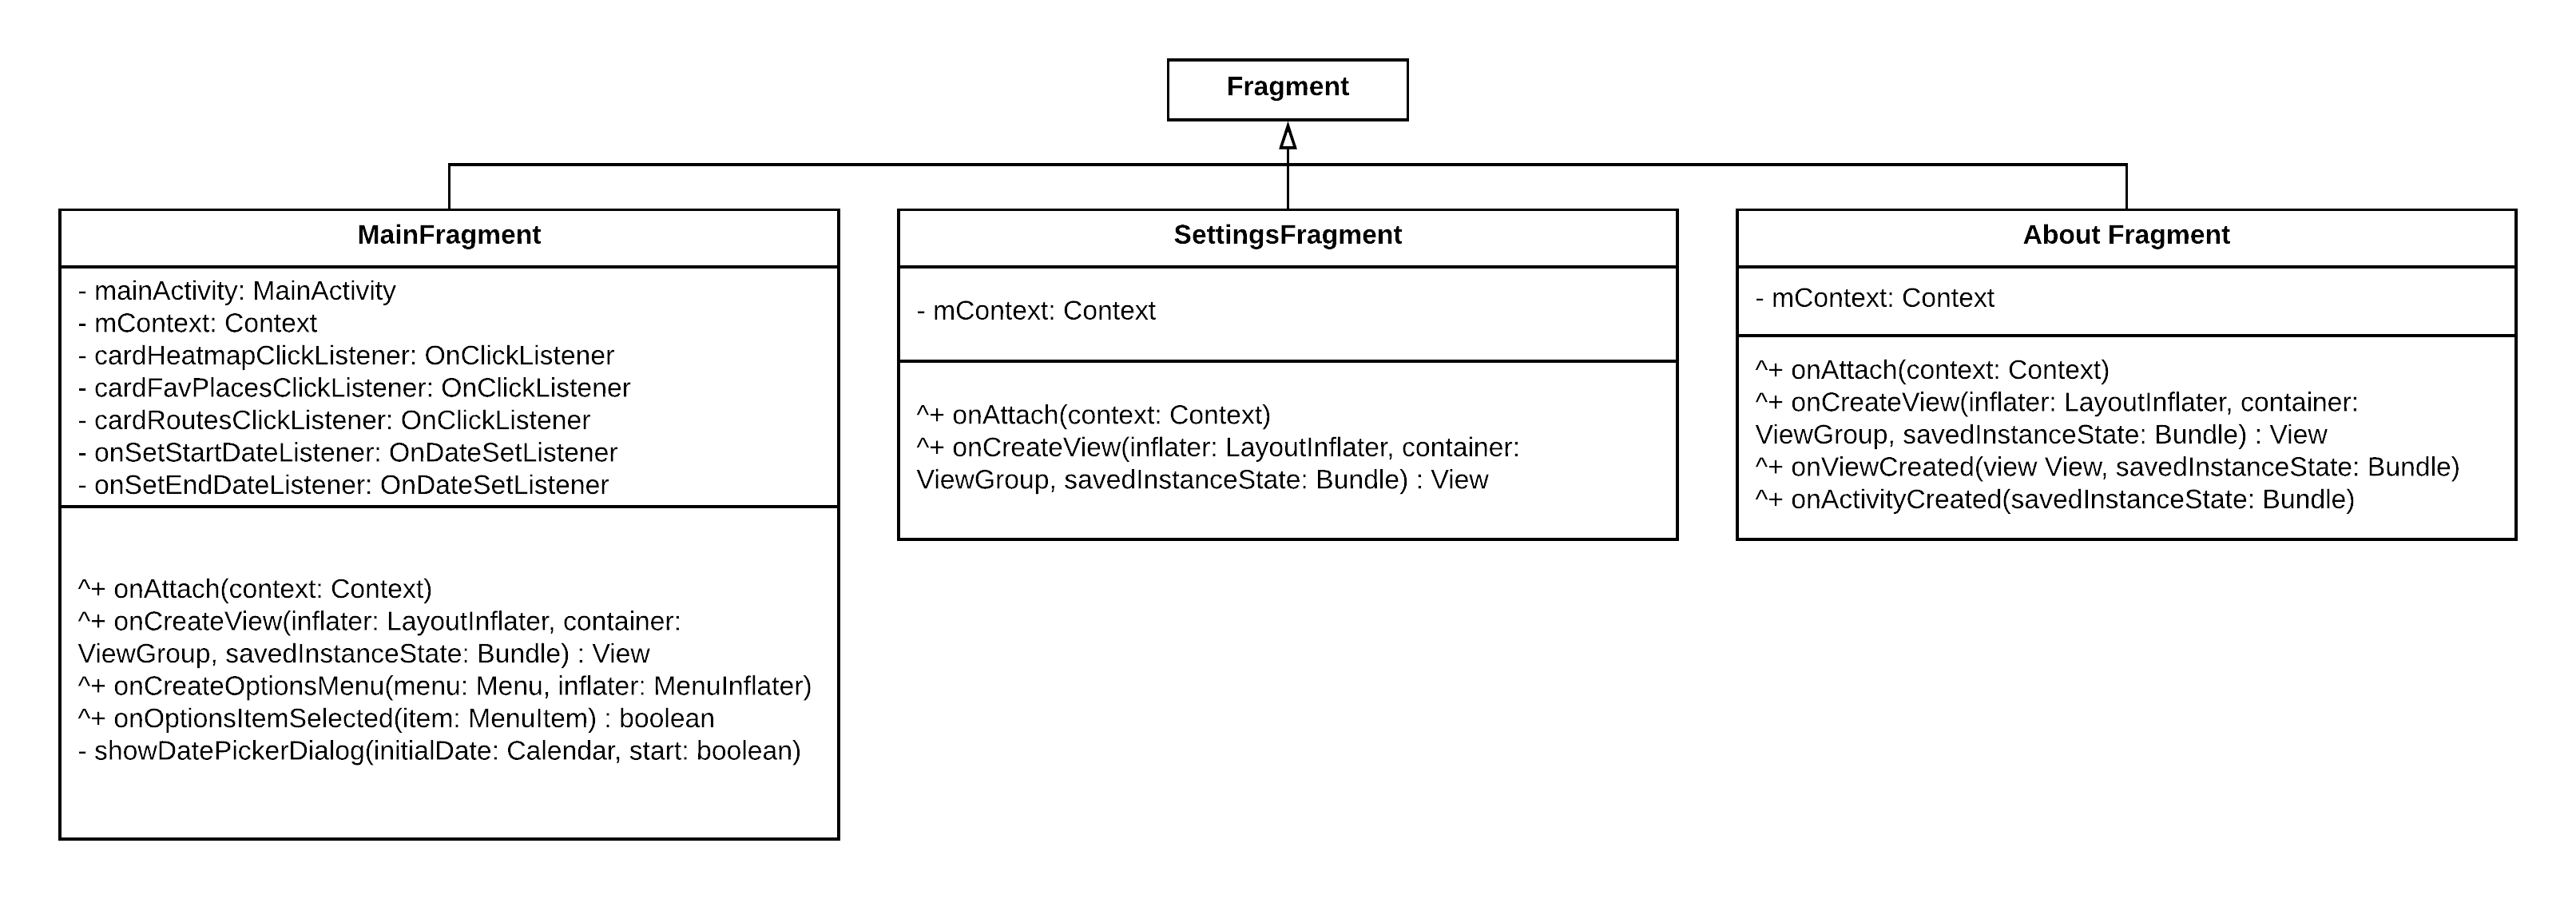
\includegraphics[width=1.0\textwidth]{class_diagram/class_diagram_2}
	    \caption{Class Diagram of Fragments}
	    \label{fig:class_diagram_fragments}
    \end{figure}
    
    The second class diagram (see Figure \ref{fig:class_diagram_fragments}) shows the three fragments that we use to display heat maps, favourite places and most frequent routes. All three of those fragments can be opened by in the \texttt{MainActivity}.
    
    \begin{figure}[H]
        \center
        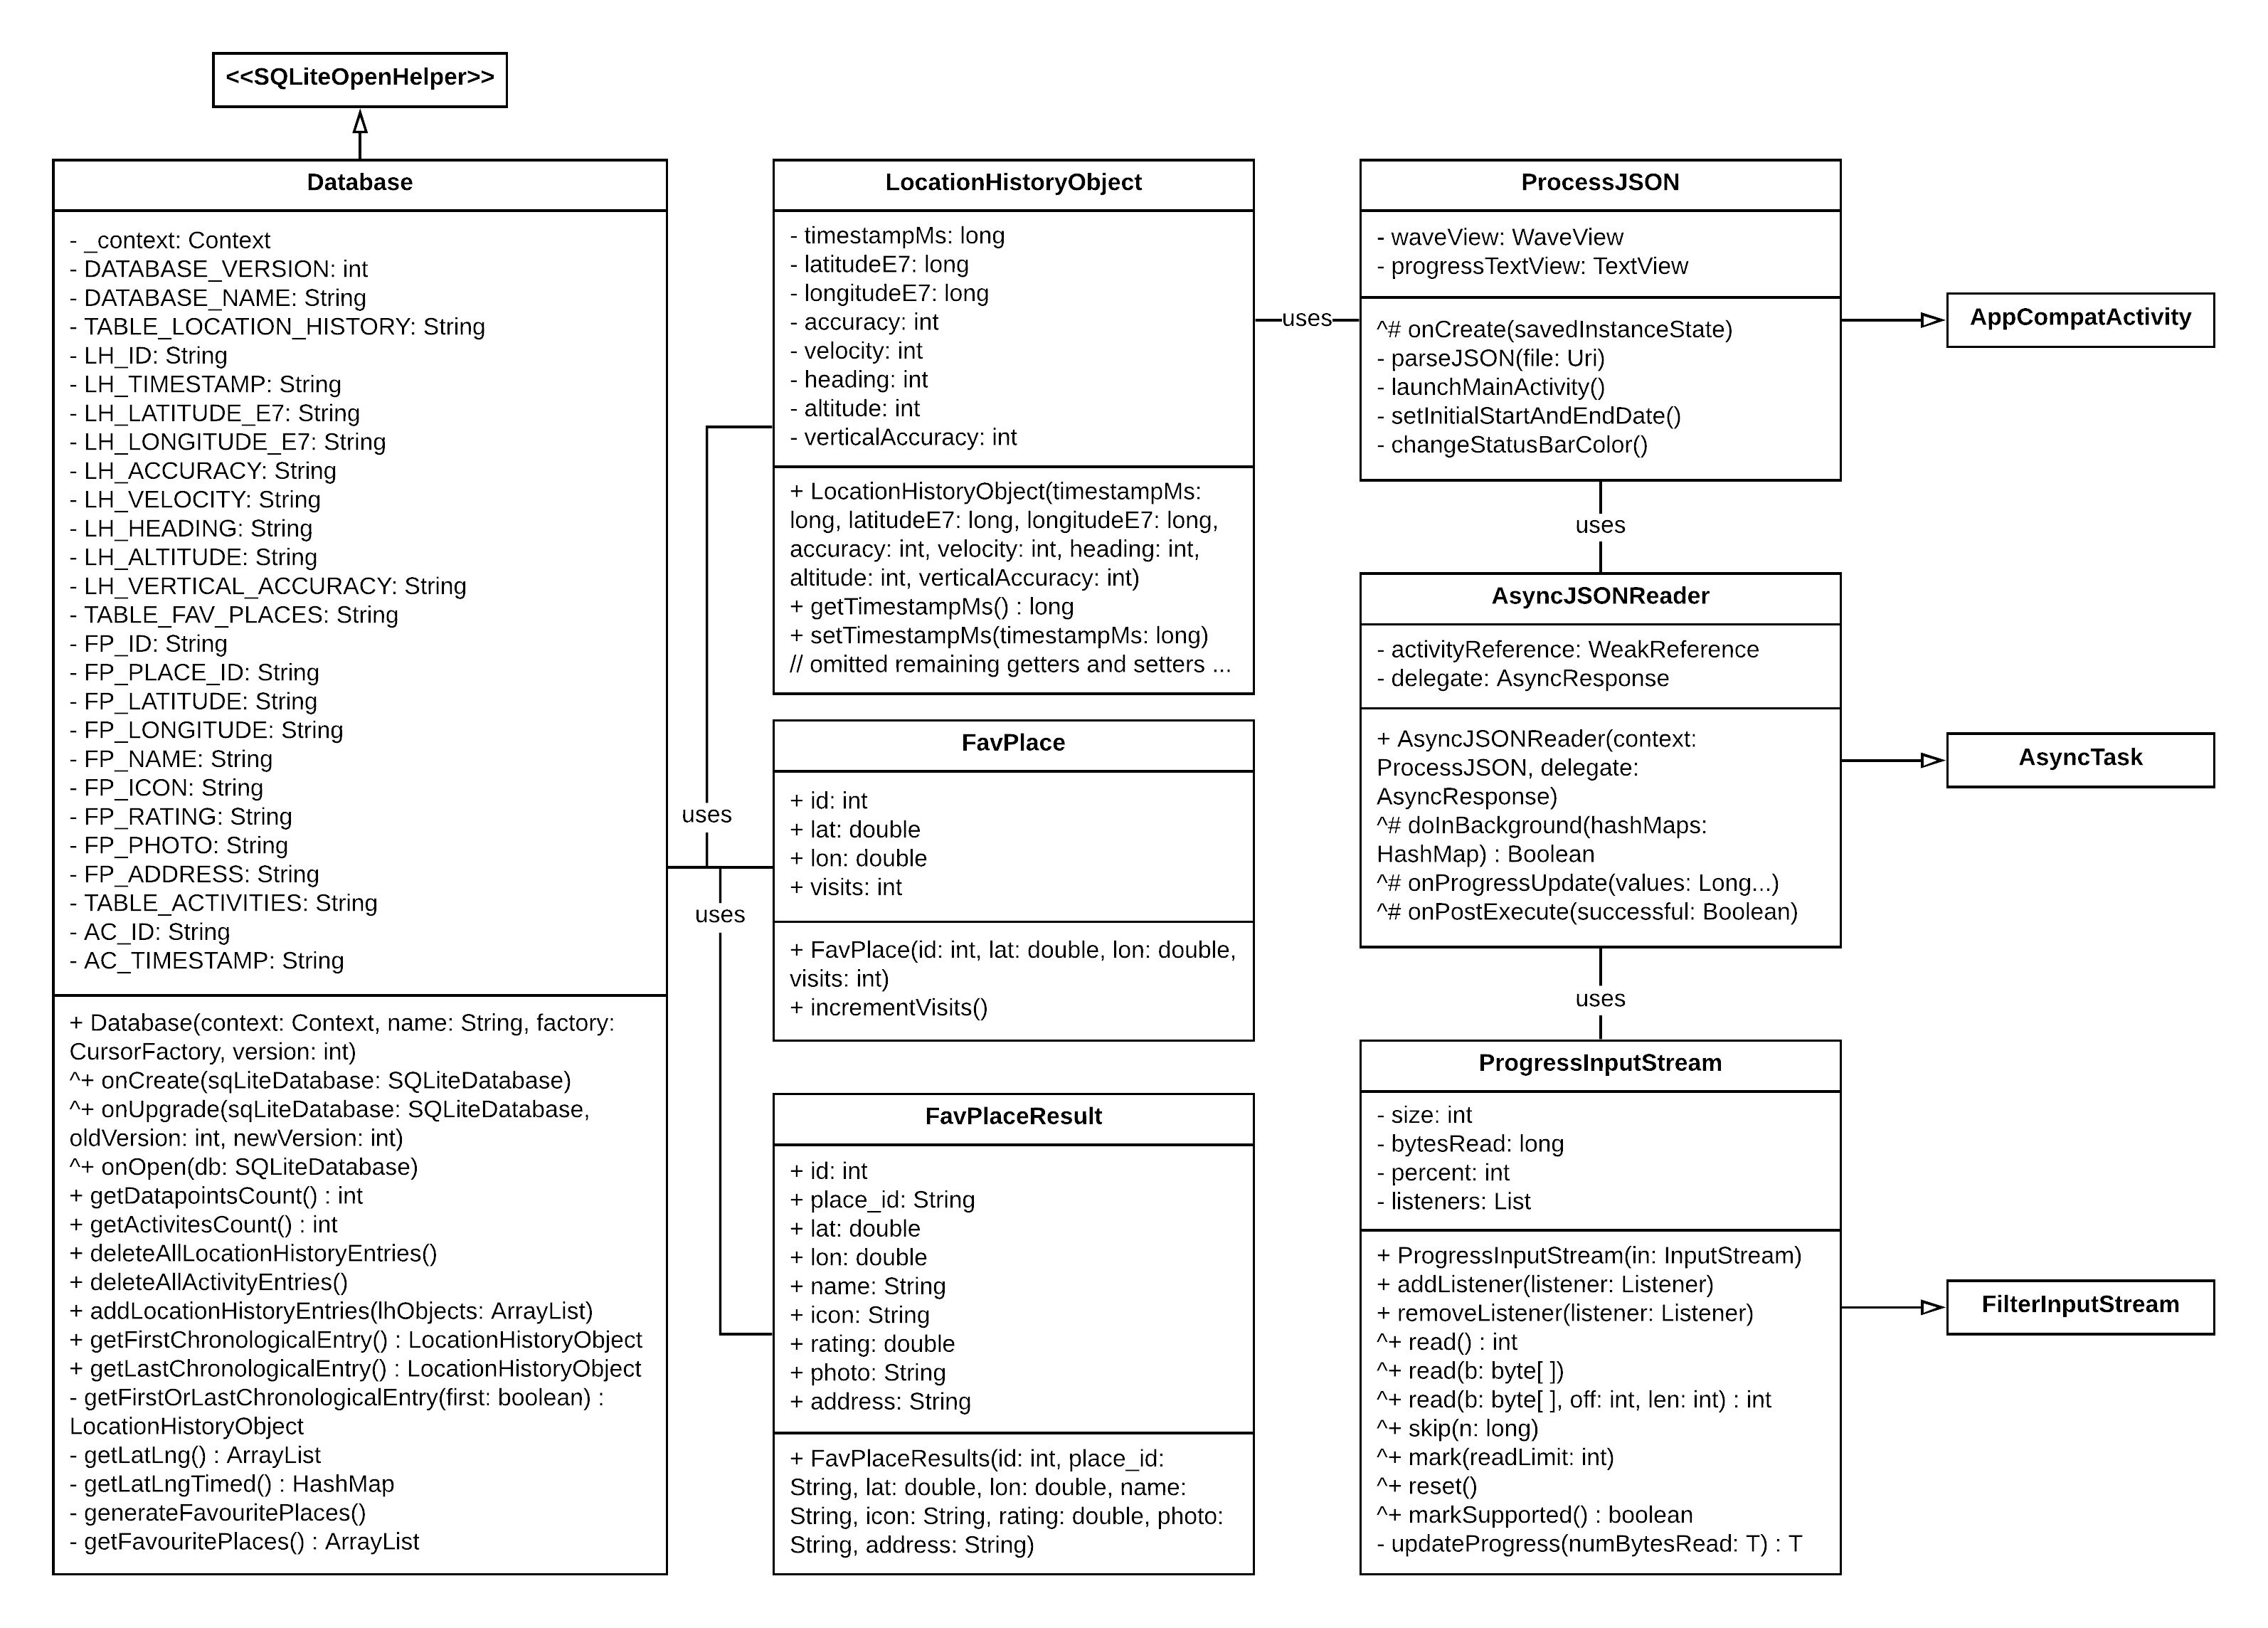
\includegraphics[width=1.0\textwidth]{class_diagram/class_diagram_3}
	    \caption{Class Diagram of Database related classes}
	    \label{fig:class_diagram_database}
    \end{figure}
    
    The third class diagram (see Figure \ref{fig:class_diagram_database}) shows all classes that are related to the database. The \texttt{Database} class itself handles creating and updating the SQLite database. To store database values in native Java objects, we use three different classes that represent certain data structures in the database. \texttt{ProcessJSON} is an activity in the application that processes a \texttt{.json} file and writes all its contents to the database. To do this, the activity uses an \texttt{AsyncTask}, which runs in the background without blocking the user interface. This asynchronous reader utilizes a custom \texttt{FilterInputStream} that shares updates on the estimated progress of the file that is being read, which is used to display a progress bar in the \texttt{ProcessJSON} activity.
    
    \begin{figure}[H]
        \center
        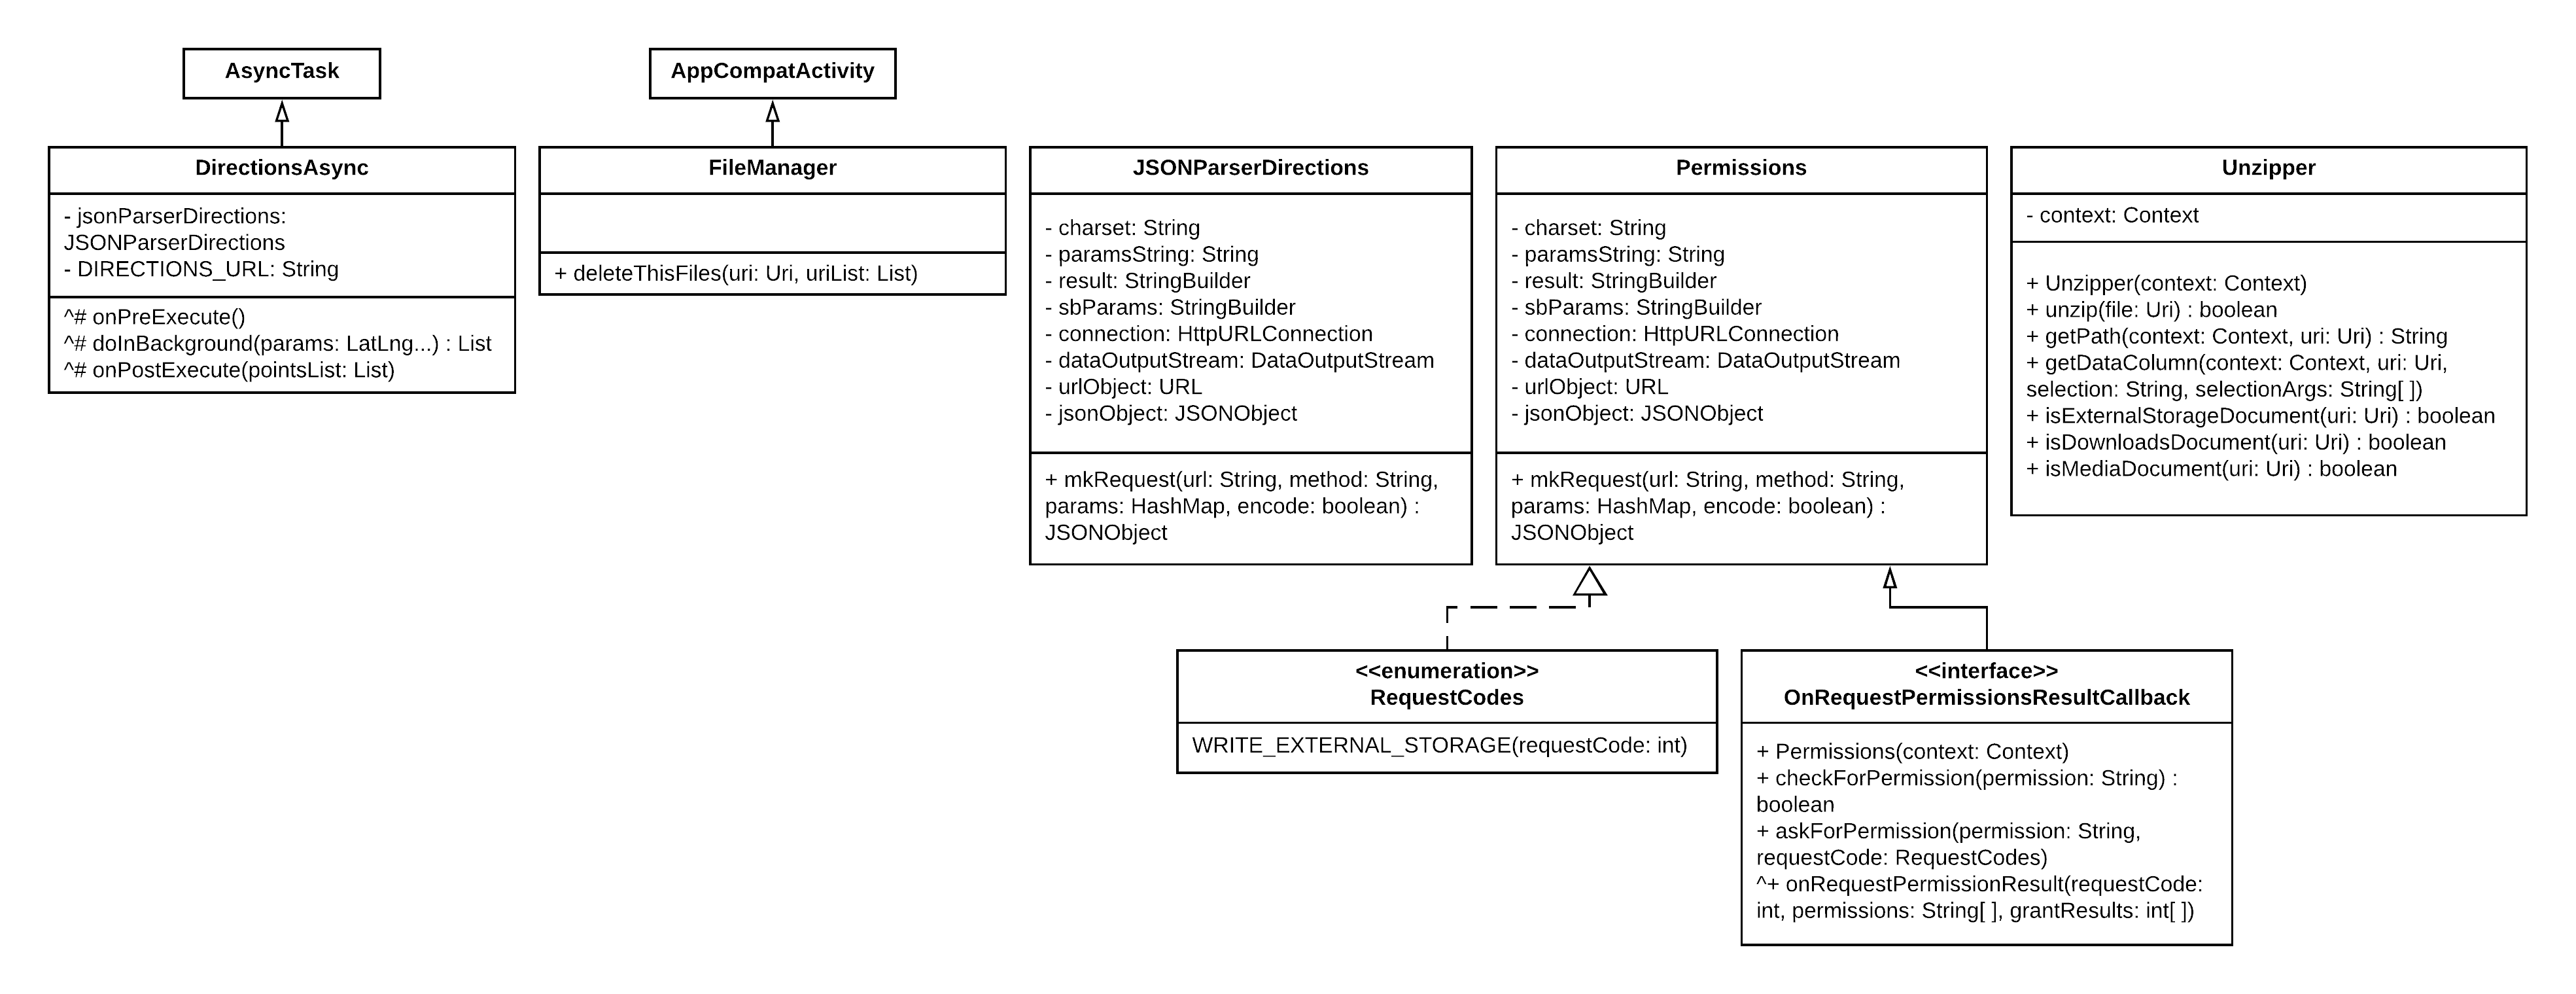
\includegraphics[width=1.0\textwidth]{class_diagram/class_diagram_4}
	    \caption{Class Diagram of Utility classes}
	    \label{fig:class_diagram_utilities}
    \end{figure}
    
    The fourth and final class diagram (see Figure \ref{fig:class_diagram_utilities}) shows classes that are used as utilities and don't have a special relationship with other parts of the application.
    
    \newpage
    \subsection{Sequence Diagram}
    Sequence diagrams show interactions between different objects, in the order they occur in \cite{SequenceDiagram}. The important thing here is in fact the sequence events happen, the actual details of the events, however they should not be omitted. The vertical axis (from top to bottom) the time sequence of events, the horizontal (from left to right) - the objects that are active at each step.
    
    \begin{figure}[H]
        \center
        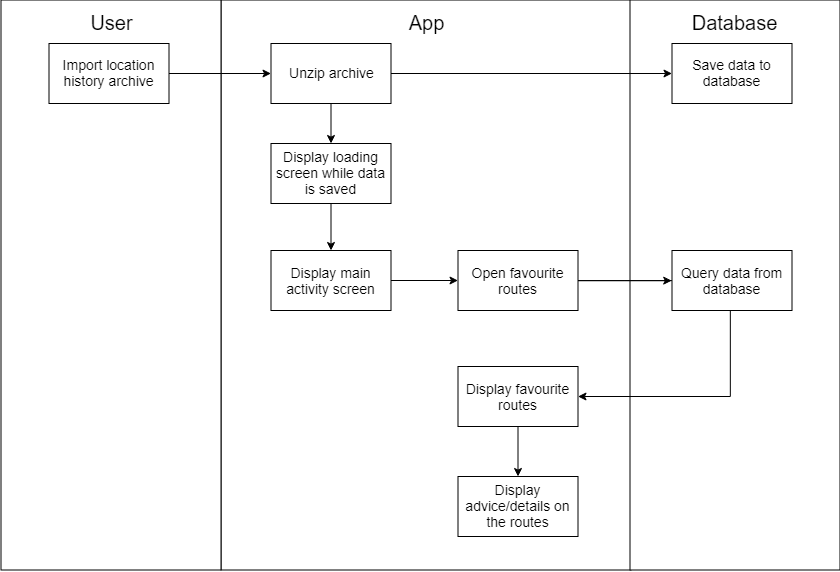
\includegraphics[width=1.0\textwidth,keepaspectratio]{pics/diagrams/SequenceDiagram.png}
	    \caption{Sequence Diagram}
    \end{figure}
    
    Our diagram shows the sequence of events that are emitted from launching Cartographer for the first time, to displaying the analysed data. The first step is for the user to import the archive containing their location history. The file is unzipped and store to the database, during which a loading screen is displayed.
    After the processing is done, the user is presented with the main screen which has 3 options to chose from - open favourite routes, favourite places or a heat map. Because the events that follow are very similar whichever option the users chooses, we included only one of them in the diagram. The use of external services was not included as it happens as a background and is not noticeable to the user.
    
    \newpage
    \subsection{Component Diagram}
    A structural diagram's purpose "is to show the structural relationships between the components of a system." \cite{ComponentDiagrams}. It can help when modelling the initial architecture of an application.
 
    \begin{figure}[H]
        \center
        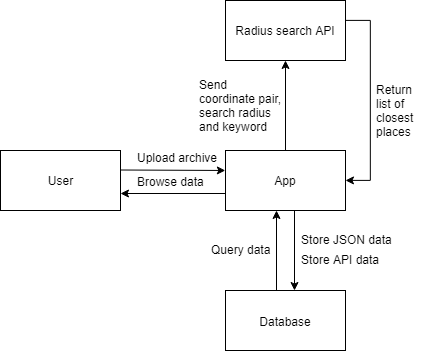
\includegraphics[width=0.8\textwidth,keepaspectratio]{pics/diagrams/ComponentDiagram.png}
	    \caption{Component Diagram}
    \end{figure}
    
    Our component diagram shows only one of the use cases of our app - the favourite places visualisation. After the archive is initially imported, it is stored in the local database. From then on data is queried from it and an external application programming interface (API) is used in order to aggregate more data, to help make the user's location history more comprehensive. Once that process is completed the user can browse the places they've visited most.
    
%----------------------------------------------------------------------------------------
%	SOFTWARE DESIGN
%----------------------------------------------------------------------------------------

\clearpage
\section{Application design} \label{sec:SoftwareDesign}
    \subsection{Introduction}
    The sketches for the application were made using the online tool \textit{Marvelapp} \cite{Marvelapp}. We chose it because it has a varied library of pre-designed components which we were able to leverage to save time. It also allows sharing the sketches, multiple people to work on them and to export them.
    For the actual components in the app we used the built-in Android library.
    
	\subsection{Introduction slides}
    \begin{figure}[ht]
        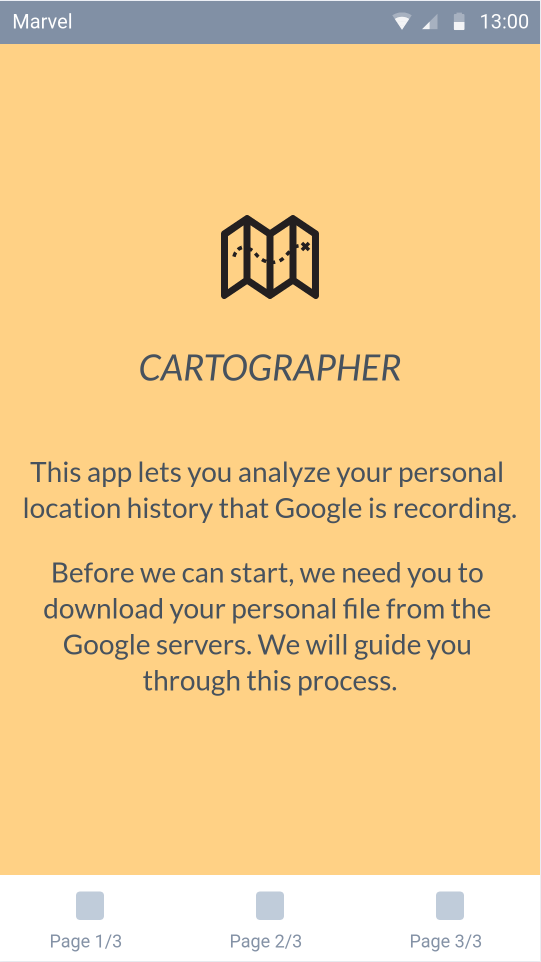
\includegraphics[height=8cm,keepaspectratio]{pics/app_design/intro.PNG}
		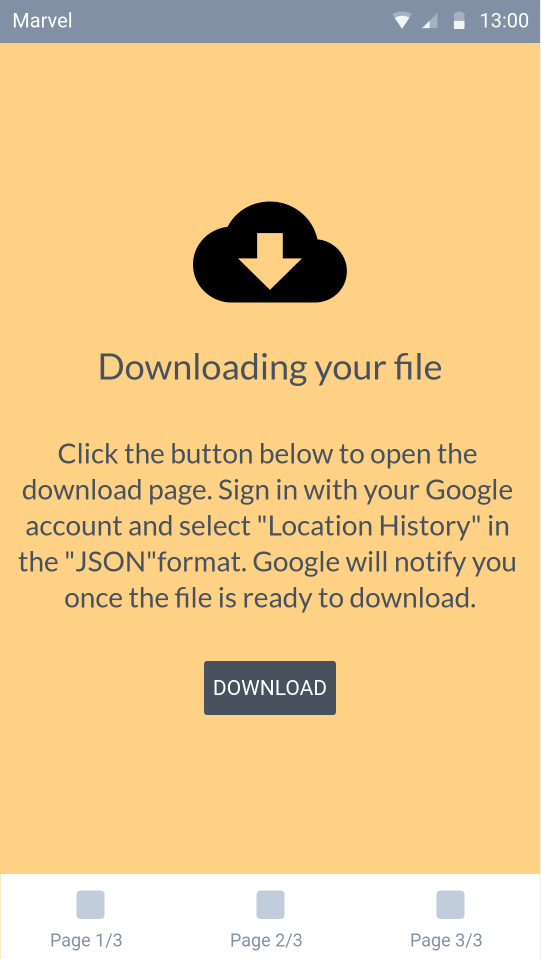
\includegraphics[height=8cm,keepaspectratio]{pics/app_design/intro2.PNG}
		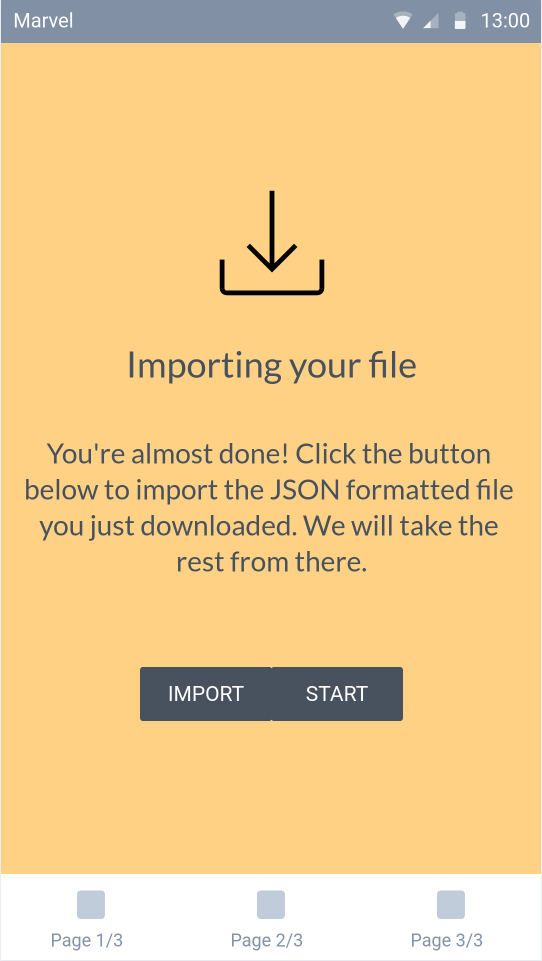
\includegraphics[height=8cm,keepaspectratio]{pics/app_design/intro3.PNG}
	    \caption{Sketch of the introduction screens}
    \end{figure}
    
    The introduction slides are only shown once, at the first start of the application. The introduction consists of several slides that show various information about the application, what it does and what it needs.
    
    The first slide informs the user of the purpose of the application and what the user is required to do. After that, three slides with more text and a button each, appears. The first slide gives the user the possibility to visit the Google web page where he or she can download the personal location history file. When downloading, Google gives users a \texttt{.zip} file, which needs to be unzipped. This is the purpose of the next slide. Here, the user can select the downloaded archive and the application will automatically unzip it. On the final slide, the user is finally asked to import the \texttt{.json} file that was contained in the archive. While processing the file, a loading screen is shown.
	
	\subsection{Main dashboard}
	\begin{figure}[ht]
	    \center
        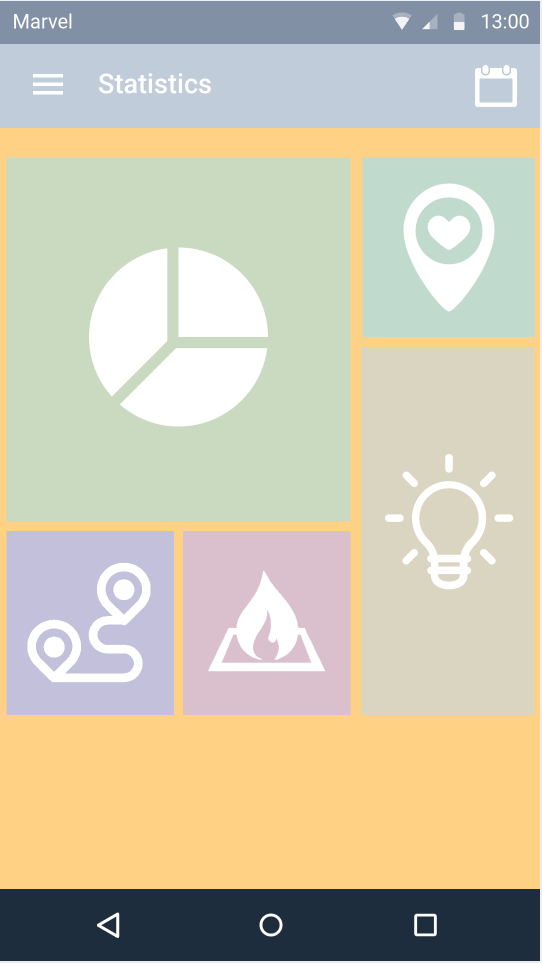
\includegraphics[height=8cm,keepaspectratio]{pics/app_design/main.PNG}
        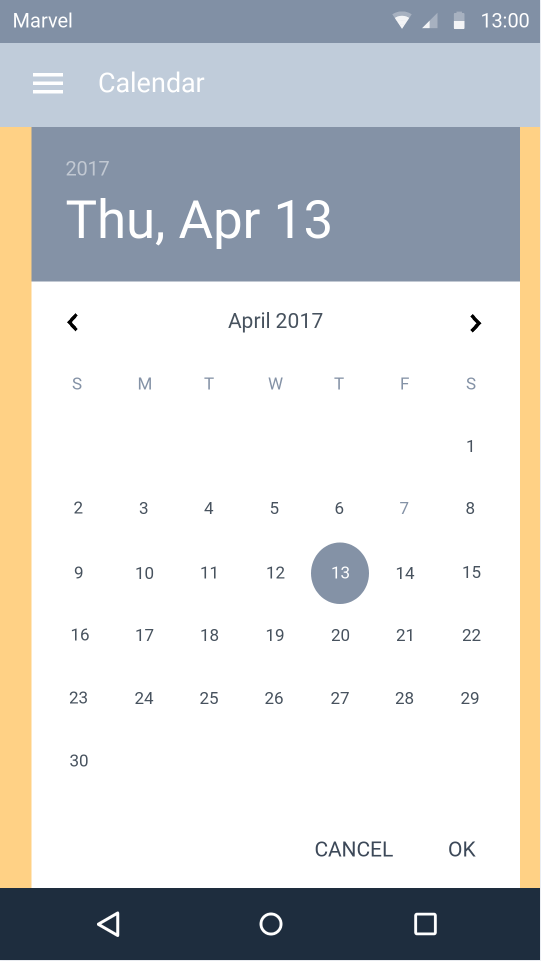
\includegraphics[height=8cm,keepaspectratio]{pics/app_design/calendar.PNG}
        \caption{Sketch of the main dashboard and calendar}
    \end{figure}
	When the user uploads his or her \texttt{.json} file and the app opens, he is directed towards a screen full of diagrams, graphs and heat maps. By pressing each one individually, he is able to access his information in a myriad of different selections: He can see how much time he has spent in different locations, he can access information on the routes he frequently travel on, how much time he spent going to said routes, how long he stays in certain locations and what transport he takes to get there, as well as the average distance he has travelled in total. In addition, he can select the calendar to change the duration of time the diagrams, graphs and heat maps take his information into account (Example: If he selects a week, the application will display his records within that week).
	
	\subsection{Favourite routes}
	In this section users can see routes they usually take. The routes are displayed as lines on a map, which are snapped to the roads.
	
	\subsection{Favourite places}
    
	There’s also an additional selection for your favourite places. By selecting that specific icon in the “Statistics”, you are able to see which locations the user most frequent, and access the information that is stored on those locations by the Google servers, such as the opening hours, contact info., distance from your location, etc.

    \begin{figure}[ht]
	    \center
        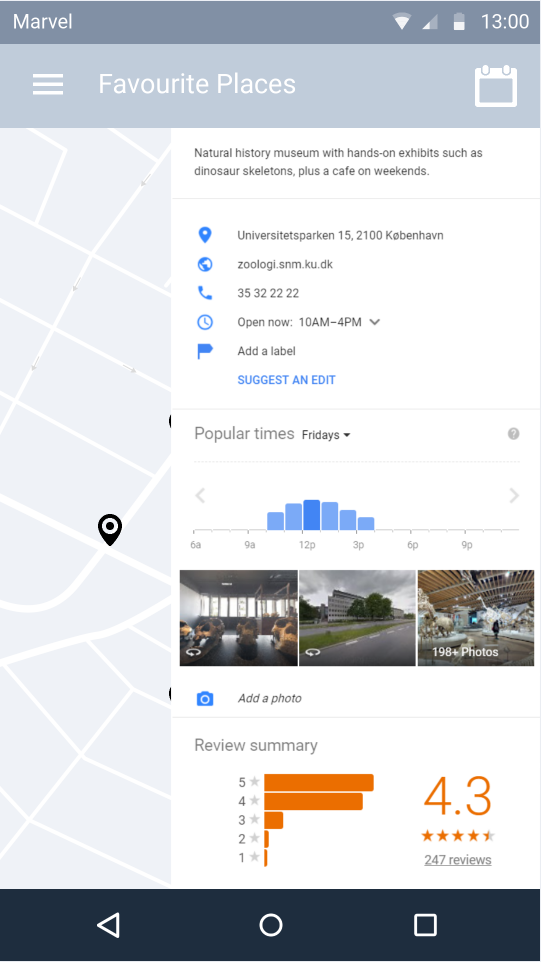
\includegraphics[height=8cm,keepaspectratio]{pics/app_design/fav_places.PNG}
        \caption{Sketch of Favourite Places}
    \end{figure}
	
	\subsection{Future implementations}
	We also wanted to provide the users with an option to access individual advice, such as what different routes could they take to get to the desired destination faster, what would be the best time to visit a specific location of choice, what other locations would the user might want to go to that would be close to their location, among many other things. Additionally, the user would be able to turn on a warning that would remind them to go outside when the app notices them to be spending too much time indoors. Unfortunately, we were not able to implement such an addition in time, but it would certainly be something we would want to do if we are ever to continue the project.

%----------------------------------------------------------------------------------------
%   IMPLEMENTATION
%----------------------------------------------------------------------------------------
    
\newpage
\section{Implementation} \label{sec:Implementation}

    \subsection{Introduction}
    We used \textit{Android Studio} as the development IDE and \textit{Java} as the main programming language. Furthermore, we used \textit{Git} for version control. The source code of this application can be viewed on \textit{GitHub} \cite{repo}.
    
    This project relies heavily on Google Application programming interfaces (API) \cite{GoogleDevProducts} and built-in Android libraries. A library we relied heavily on was the Java Client for Google Maps Services \cite{JavaGoogleAPI}. Most of the APIs Google offers are intended to be used as JavaScript services, however, the aforementioned library adds a Java client which provides access to the API endpoints.
    Due to the absence of funds when creating this project we were forced to use the free versions of Google's APIs which have usage quotas. The Geocoding API, for example, is limited to
    \cite{GeoCodingAPILimits}:
    
    \begin{itemize}
        \item 2,500 free requests per day, calculated as the sum of client-side and server-side queries
        \item 50 requests per second, calculated as the sum of client-side and server-side queries
    \end{itemize}
    
    Considering that it's expected four users to have in excess of 100000 coordinates recorded (the amount depends on the individual user's settings), these limits make the app very slow and limits its capabilities. Nevertheless, the APIs provided a quick and easy way to implement the features we wanted to include in a usable manner.
    
    \subsection{Location history archive} \label{sec:JsonFile}
    The user uploads their location history archive as a \texttt{.zip} \cite{zip} file, which contains a \texttt{.json} \cite{json} file. The JSON contains a list of objects, each containing a time stamp, latitude, longitude and accuracy of the coordinates. Some objects also include the activity, that Google has calculated, as a list of objects, containing the type and confidence of the estimate. Very few objects have values such as altitude, velocity and heading (in degrees). In the example below there is an 88\% chance that the device was not moving when the data was recorded. This is an example of the objects in the JSON: 
    
    \begin{minted}[frame=single,framesep=3mm,linenos=true,tabsize=4]{js}
{
    timestampMs: '1521182781172',
    latitudeE7: 556483768,
    longitudeE7: 125526238,
    accuracy: 17
},
{
    timestampMs: '1521182815388',
    latitudeE7: 556483816,
    longitudeE7: 125526142,
    accuracy: 17,
    activity: [
      {
        timestampMs: '1521182807100',
        activity: [
          {
            type: 'STILL',
            confidence: 88
          },
          {
            type: 'IN_VEHICLE',
            confidence: 4
          },
          {
            type: 'IN_ROAD_VEHICLE',
            confidence: 4
          },
          {
            type: 'UNKNOWN',
            confidence: 3
          },
          {
            type: 'IN_RAIL_VEHICLE',
            confidence: 3
          },
          {
            type: 'ON_FOOT',
            confidence: 2
          },
          {
            type: 'WALKING',
            confidence: 2
          }
        ]
      }
    ]
}
    \end{minted}
    
    \subsection{Introduction slides}
    
    \begin{figure}[ht]
	    \center
        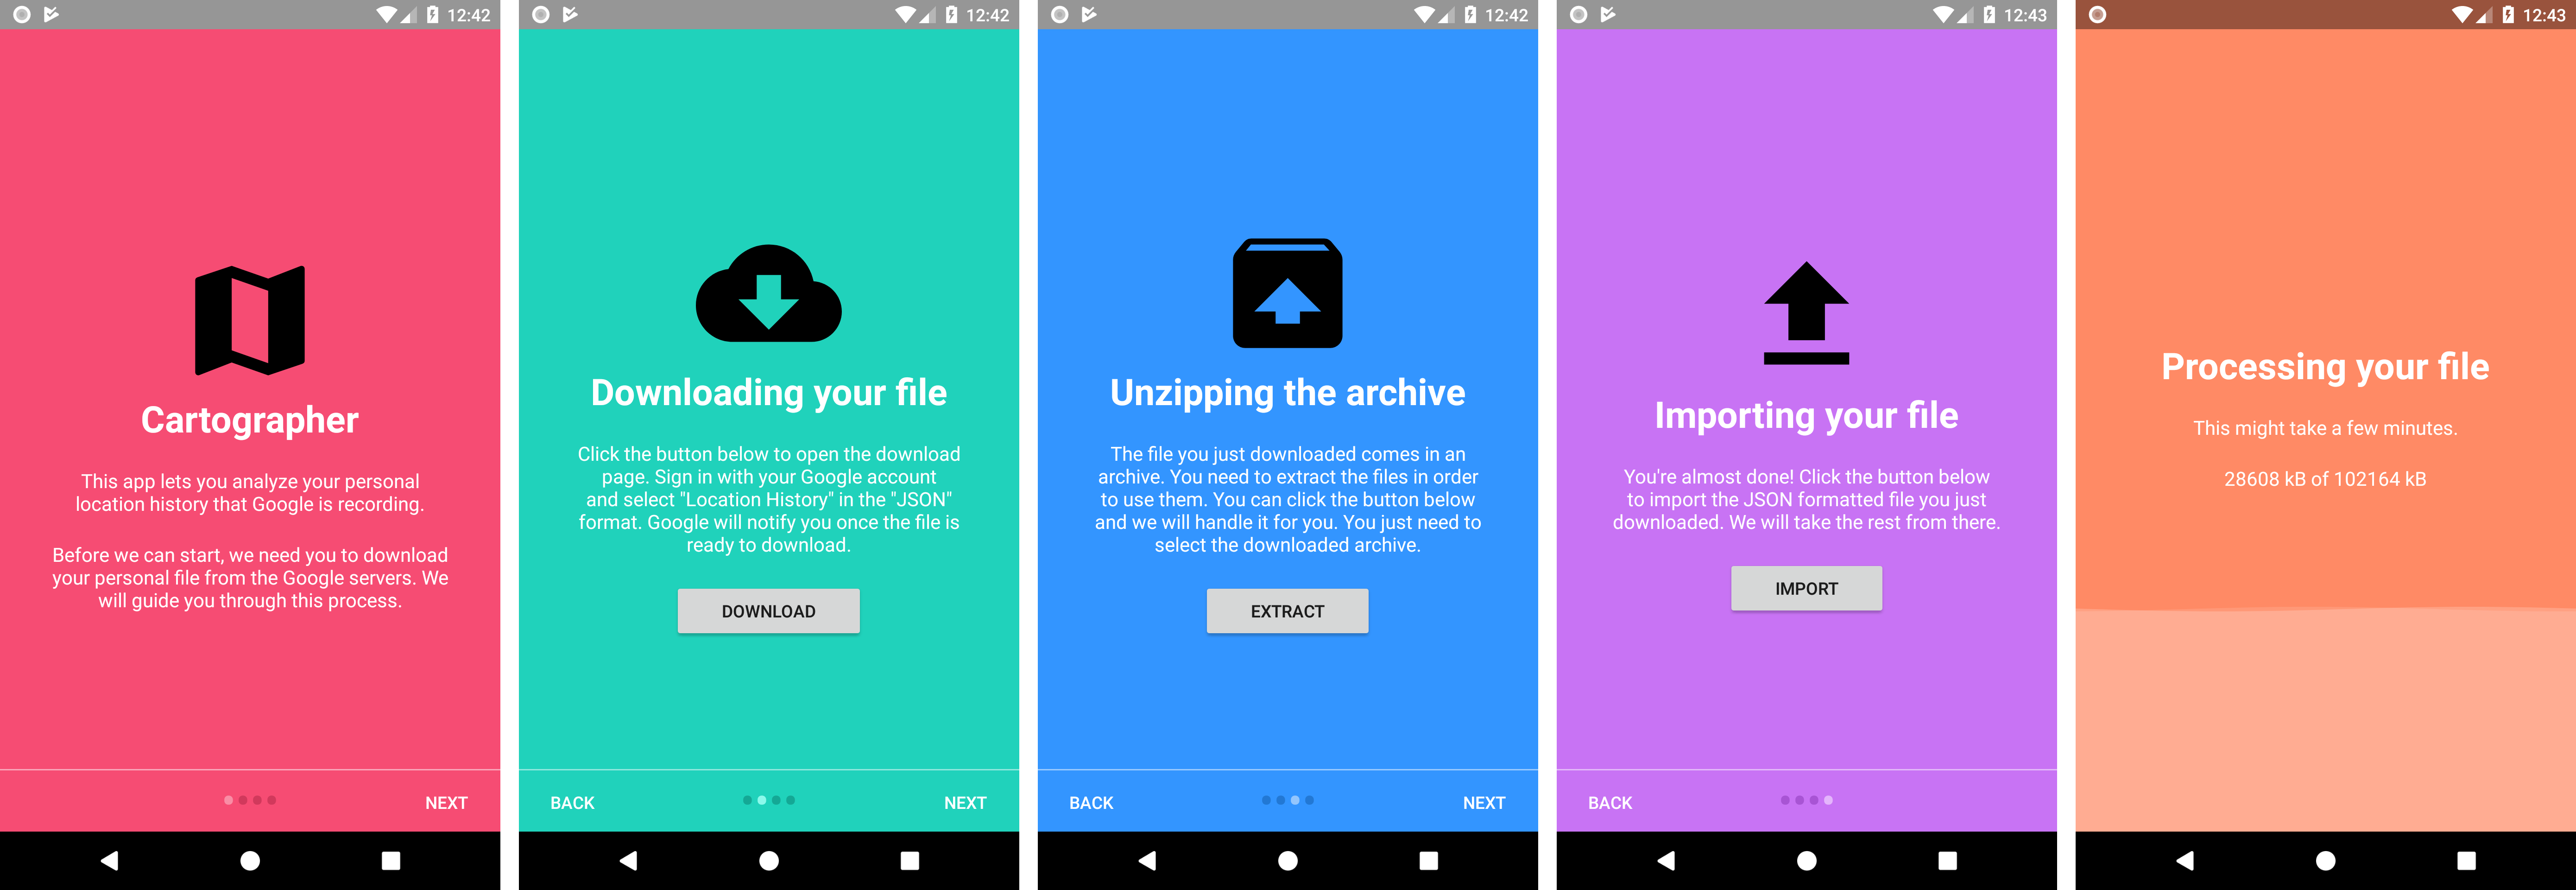
\includegraphics[width=1\textwidth]{pics/app_design/intro_slides_comp}
        \caption{Introduction slides}
        \label{fig:introduction_slides}
    \end{figure}
    
    There are many Android libraries for introduction slides, such as \textit{AppIntro} \cite{AppIntro} or \textit{Material Intro Screen} \cite{MaterialIntroScreen}. However, while testing out those two libraries, among others, we quickly noticed some problems regarding bugs and usability, as well as the fact that some libraries are outdated and should therefore not be used. 
    
    An alternative was quickly found in a tutorial on \textit{Android Hive} \cite{IntroSlidesTutorial} that shows how to implement your own, custom introduction slides. This helped us a lot with setting up the slides. However, we changed several parts of the source code from the tutorial. For example, we didn't want to have a \textit{Skip} button, because the user is required to upload a file before he or she can proceed. Because of this, we reworked this button to be a \textit{Back} button. All final slides can be seen in Figure \ref{fig:introduction_slides}.
    
    The custom introduction slides also caused some issues with the \texttt{ViewPager} widget, because the UI elements on some slides were visible, but not accessible. This was caused by the \texttt{ViewPager} not caching the next slide when navigating with the buttons instead of swiping. This took a long time to fix and we finally discovered that we can just preload every slide into the memory, instead of dynamically loading it on demand. This fixed our issue.
    
    As for the functionality of the slides, the \textit{Download} button opens the default browser and navigates to the Google Takeout page, which is the central repository where users can download their Google data.
    
    The \textit{Extract} button on the third slide opens a file browser and asks the user to select a \texttt{.zip} file, which will then be extracted to the same directory. For this, we used the Java library \textit{Zip4j} \cite{zip4j}.
    
    Finally, the \textit{Import} button on the last slide opens yet another file browser to select the \texttt{.json} file, which will then be processed by the app. Because the size of this file is usually of significant size ($\sim$100 MB for one year of data), a separate loading screen is shown while the file is being processed in the background. The loading animation in the background is a wave that is progressively filling up the screen while progressing. This widget is coming from the \textit{Wave View} library \cite{WaveView}.
    
    \subsection{File processing}
    
    Processing the JSON file was certainly one of the most difficult programming tasks in the project. The file usually contains millions of lines of text and can be several hundreds of megabytes large. We had to find a way to parse this file fast without annoying the user if the process is too slow.
    
    There are many JSON libraries for Java, such as \textit{Jackson} \cite{Jackson},  \textit{GSON} \cite{Gson} and the native Java APIs \cite{JavaJsonNative} that can help us in this task. We decided to use \textit{Gson} because we found it to be the easiest to use. Furthermore, it is developed by Google, which means that is should work well with Android OS. Because of this, we are comfortable with using their library instead of others.
    
    A big problem with parsing such a big file is the memory. It is not possible to simply use the built-in functions of the library to read the whole file into the memory and receive some kind of output. This is highly inefficient and crashes the app if the file is too large. Because of this, we are using the \texttt{Json Reader} of the Gson library, which lets us read a JSON file token by token and decide ourselves, what to do with the values.
    
    This process is running in an asynchronous task so that the UI is not blocked and the loading screen can be updated. Another issue here was that we needed to calculate a percentage value of the progress in order to show it on the loading screen. The normal \texttt{Input Stream} in Java does not implement such a functionality, but we found a solution online \cite{ProgressInputStream}. This solution simply extended the normal \texttt{Input Stream} in Java and added a method to estimate the progress, by counting the processed bytes and dividing it by the full file size.
    
    The following code snippet shows how the application reads the \texttt{.json} file and converts them to Java objects. The structure of the JSON file can be seen in section \ref{sec:JsonFile}. It consumes the file token by token, reads the relevant information from each object, converts them to Java objects and finally puts them in the local database.
    
\begin{minted}[linenos,breaklines]{java}
com.google.gson.stream.JsonReader jsonReader = new com.google.gson.stream.JsonReader(new InputStreamReader(progressInputStream));

if (jsonReader.hasNext() && jsonReader.peek().equals(JsonToken.BEGIN_OBJECT)) {
    jsonReader.beginObject(); 
    if (jsonReader.hasNext() && jsonReader.peek().equals(JsonToken.NAME)) { 
        String firstObjectName = jsonReader.nextName(); 
        if (firstObjectName.equals("locations") && jsonReader.hasNext() && jsonReader.peek().equals(JsonToken.BEGIN_ARRAY)) { 
            jsonReader.beginArray(); 

            ArrayList<LocationHistoryObject> parsedObjects = new ArrayList<>();
            boolean hasAnotherObjectInArray = true;
            while (hasAnotherObjectInArray) { 
                if (jsonReader.peek().equals(JsonToken.BEGIN_OBJECT)) {
                    jsonReader.beginObject();

                    LocationHistoryObject currentObject = new LocationHistoryObject();

                    while (jsonReader.hasNext()) {
                        if (jsonReader.peek().equals(JsonToken.NAME)) {
                            String nextName = jsonReader.nextName();
                            switch (nextName) {
                                case "timestampMs": 
                                    currentObject.setTimestampMs(Long.parseLong( jsonReader.nextString()));
                                    Log.i("timestampMs", String.valueOf(currentObject.getTimestampMs()));
                                    break;
                                // omitted remaining cases ...
                            }
                        }
                    }

                    jsonReader.endObject();
                    hasAnotherObjectInArray = jsonReader.peek().equals(JsonToken.BEGIN_OBJECT); 

                    if (parsedObjects.size() < 1024) {
                        parsedObjects.add(currentObject);
                    } else {        
                        database.addLocationHistoryEntries(parsedObjects);
                        parsedObjects.clear();
                    }
                }
            }

            if (parsedObjects.size() > 0) {
                database.addLocationHistoryEntries(parsedObjects);
            }

            if (jsonReader.peek().equals(JsonToken.END_ARRAY)) {
                jsonReader.endArray();
            }
        }
    }

    if (jsonReader.peek().equals(JsonToken.END_OBJECT)) { 
        jsonReader.endObject();
    }
}
jsonReader.close();

Log.i("Entry count", String.valueOf(database.getDatapointsCount()));
\end{minted}
    
    \subsection{Database}
    
    The application stores the data from the user's JSON file in a database to have it available fast. Parsing the JSON file over and over again when the user requests to see the heat map, for example, is highly inefficient.
    
    We chose SQLite as our database for several reasons. First of all, the database needs to be offline in order to comply with the entire project. It would be hypocritical to promote privacy on one hand, but then go ahead and store all the user's highly sensitive data online. There are plenty of offline databases available for Java/Android, but we only needed a simple way of storing the massive amount of data and be able to query it quickly again. We would have liked to use \textit{Realm} \cite{Realm}, but it is not available for free. The advantages of \textit{Realm} are that you can work with native objects instead of reading and writing single values from and to columns (as in SQL), as well as being able to easily encrypt the database with AES-256 encryption \cite{RealmFeatures}, which would be a big benefit to us, since we want to store the sensitive data as securely as possible. However, because it is not free, we stuck to SQLite due to its ease of use and high popularity, which means that there is plenty of documentation and support online.
    
    The database consists of several tables. The biggest and most important table is the entire data from the user's JSON file. This data is identical to the file's content, but available much faster because it is stored in a database and not the file. There are also smaller tables for features such as the favourite places. This table is being used to store the processed information from the main table so that not all data has to be analysed over and over again when using a feature.
    
    \subsection{Heatmap}
    
    \subsection{Favourite places}
    
    \begin{figure}[ht]
        \center
        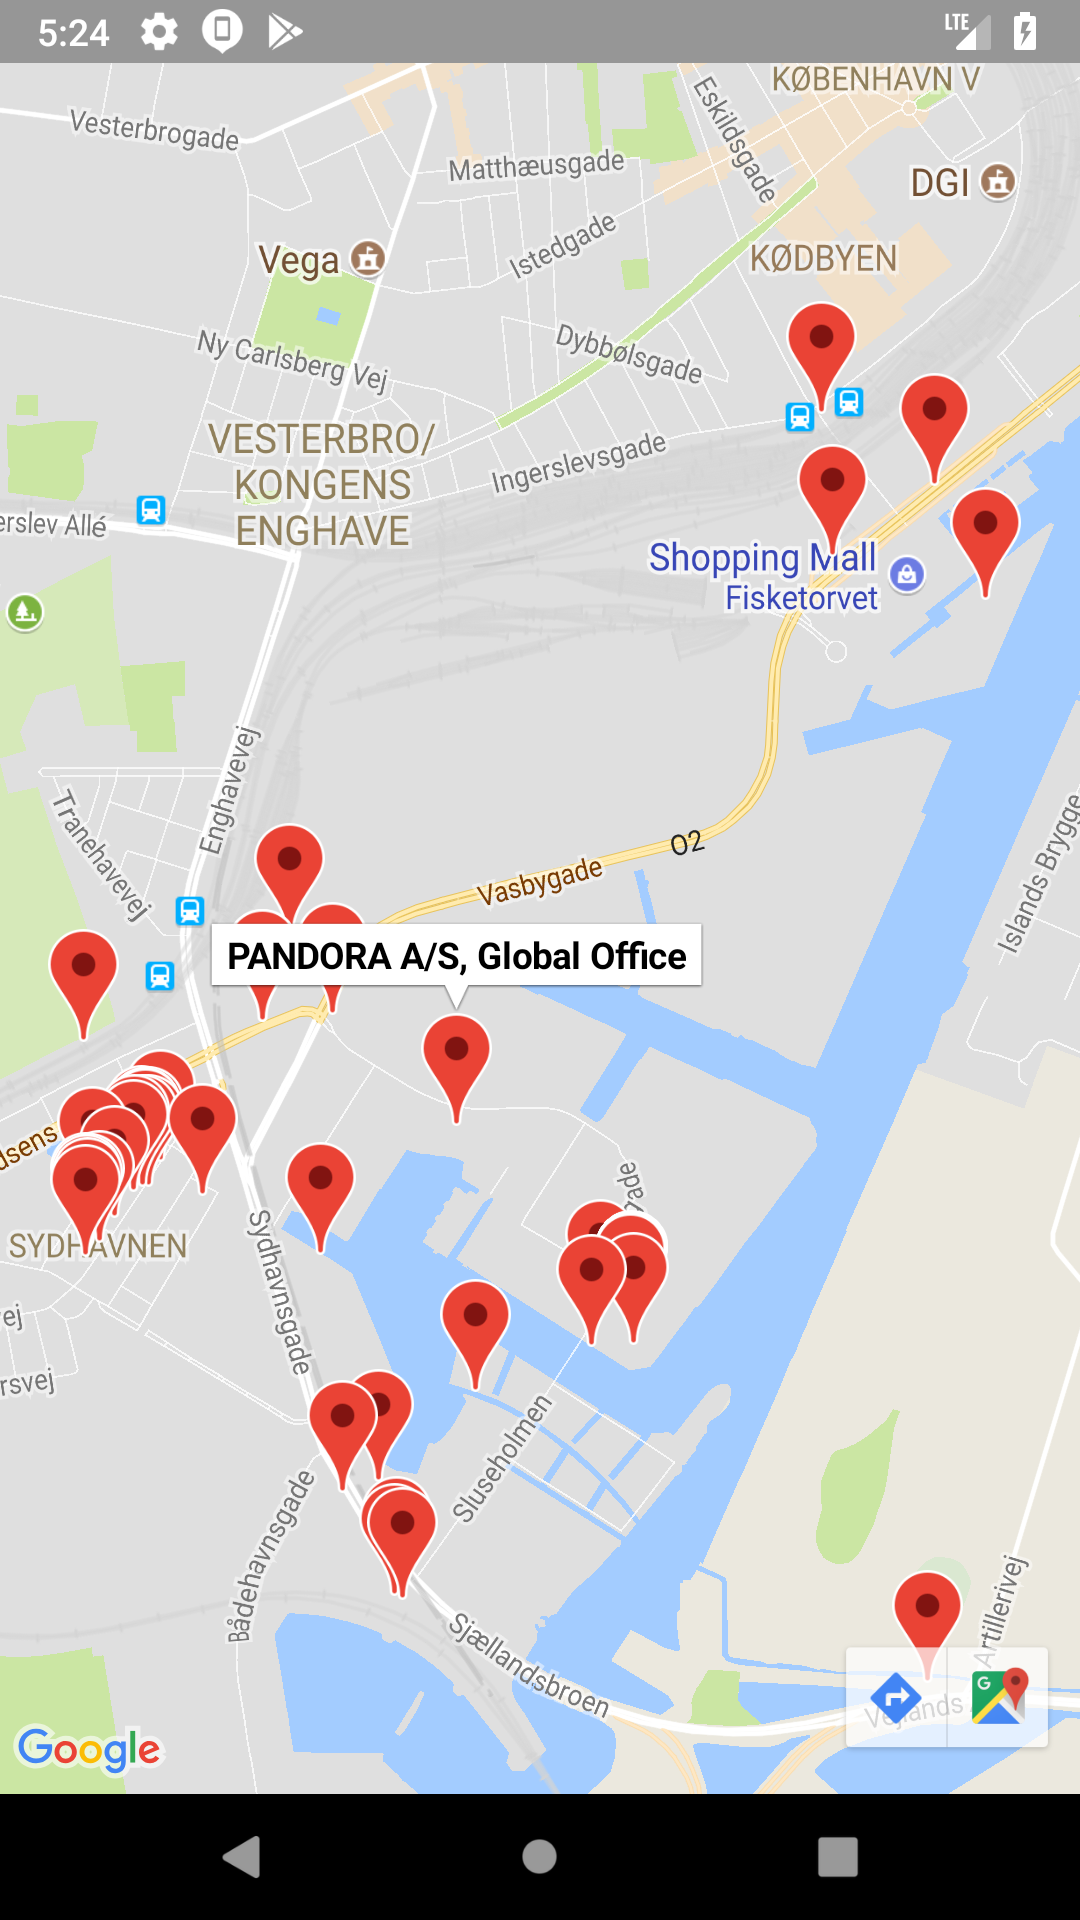
\includegraphics[height=8cm,keepaspectratio]{pics/fav-places-screenshot.png}
        \caption{Screenshot of Favourite Places}
    \end{figure}
    To generate the list of favourite places we had to go through all the data points a user has, check if some of them are duplicated and how many times. The data provided by the user though contains only the coordinates where they have been. To find out if they were actually in some kind of establishment (restaurant, supermarket, shopping mall, etc) we need to find out what places are nearby the user. 
    
    We accomplished this by using Google's Radar Search API \cite{GoogleRadarSearch}. It works by passing it a coordinate to the API and it returns a list of businesses that are near those coordinates. Along with the latitude and longitude, you must specify the radius around the coordinate the API will search along with a keyword, name or type \cite{GoogleAPISupportedTypes}. We chose to pass a keyword parameter, with the value of "a", because it's a popular letter in the English language and we wanted to get the largest amount of results possible.
    
\begin{minted}[linenos,breaklines]{java}
PlacesSearchResponse result = PlacesApi.nearbySearchQuery(context, new LatLng(place.lat, place.lon)).radius(1000).keyword("a").await();

ContentValues favPlaceRow = new ContentValues();
if (result.results.length > 0) {
    favPlaceRow.put(FP_ID, place.id);
    favPlaceRow.put(FP_PLACE_ID, result.results[0].placeId);
    favPlaceRow.put(FP_LATITUDE, place.lat);
    favPlaceRow.put(FP_LONGITUDE, place.lon);
    favPlaceRow.put(FP_NAME, result.results[0].name);
    favPlaceRow.put(FP_ICON, String.valueOf(result.results[0].icon));
    favPlaceRow.put(FP_RATING, result.results[0].rating);
    favPlaceRow.put(FP_PHOTO, String.valueOf(result.results[0].photos[0]));
    favPlaceRow.put(FP_ADDRESS, result.results[0].vicinity);
    db.insert(TABLE_FAV_PLACES, null, favPlaceRow);
}
\end{minted}
    
    The most relevant result is stored in a table for all the favourite places, which is queried when rendering the favourite places view and the results are rendered as markers on a map. When a marker has been clicked, the name of the business located there is displayed.
    
    \subsection{Routes}
    
    \newpage
    
    \subsection{Authentication}
    
    The implementation of authentication is rather like a sketch of it, because security was not our goal and task. Due to this, it is placed in separate, Authentication branch. There are 3 main activities: LoginActivity, RegisterActivity and UserAreaActivity. There are also 3 .xml files with layouts to visualize them.
    
    \subsubsection{Register activity and register request}
        
    \begin{figure}[ht]
      \center
      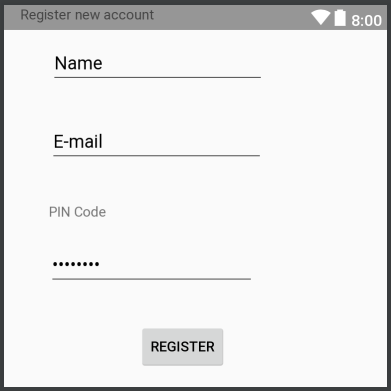
\includegraphics[width=0.4\textwidth]{authentication/register.png}
      \caption{Registration page}
      \label{fig:registration_page}
    \end{figure}
    
    RegisterActivity and RegisterRequest are two classes that are related to each other. RegisterActivity task is to collect user data (email, name and pin code) and then by pressing "Register" button it is calling RegisterRequest method(that is in RegisterRequest class). This method is handling creation of the request for the Register.php file using Volley library \cite{VolleyLibrary}.
    
    \begin{figure}[ht]
      \center
      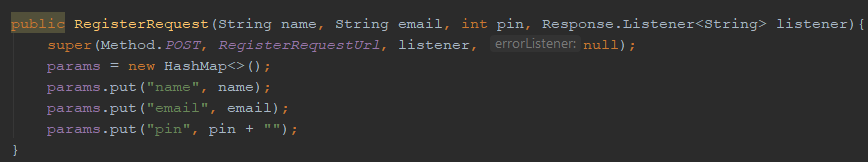
\includegraphics[width=0.9\textwidth]{authentication/registerRequest.png}
      \caption{Register request method}
      \label{fig:register_request}
    \end{figure}
    
    \subsubsection{Server and database}
    
    The server is created on hostinger.com website and the url to it is: cartographer.com. On this server we have two .php files: Login.php and Register.php. By these files we have created the connection with a database. The database is made on the same hosting and contains one table called 'user'. In this table we have 4 fields: auto-incremented intiger 'userID', varchar 'name', varchar 'email' and integer 'pin'. This database is made to store user data inserted during registration process.
    
    
    \begin{figure}[ht]
      \center
      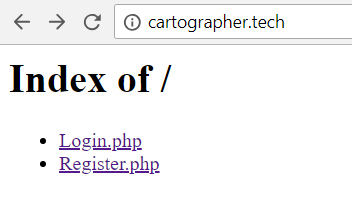
\includegraphics[width=0.4\textwidth]{authentication/server.png}
      \caption{PHP files on cartographer.com}
      \label{fig:register_request}
    \end{figure}

    \subsubsection{Login activity and login request}
    
    Login activity class contains two EditText variables and one button. This button has set onClickListener. This listener is waiting to receive a message "success", if the data that user put in are correct. If it does, then it is displaying the name of the user. If not, then the alert dialog shows up with the message that login failed. LoginRequest class includes method that creates the request for Login.php file.
    
    \subsection{Conclusion}

%----------------------------------------------------------------------------------------
%   USER RESEARCH
%----------------------------------------------------------------------------------------

\newpage
\section{User Research} \label{sec:UserResearch}

The online survey, which was described in the Methodology, received about 50 answers, three weeks after publishing. There are no statistics of where participants come from, what their background is or what their age is. However, we can make an educated guess that around half the answers are from AAU students (because the survey was shared mainly with fellow students), and the other half from unknown persons that participated through one of the websites described in the Methodology. We can guess this, because there was a delay of a few days between posting the survey in the AAU project help Facebook group and submitting it to third party online survey services.

\subsection{Android and Google Maps}

The first step of the survey is to filter out irrelevant participants. Since this project is all about creating an Android application, we are mainly looking for Android users. However, other smartphone users are still relevant, if they use the Google Maps mobile app. Despite the Android market share of 75\% in 2017 \cite{SmartphoneOSMarketShare}, most participants were not Android users. In fact, only 22 out of 47 participants (46,8\%) were using that operating system. This is most likely due to the higher market share of iOS in Denmark \cite{SmartphoneOSMarketShareDenmark} and the fact that most of our participants reside in Denmark.

Out of the 25 non-Android users, only 4 participants answered that they don't have the Google Maps mobile application installed on their phone. In total, only 4 out of 47 (around 8\%) were irrelevant for the survey.

\subsection{Knowledge of location related data collection}

\begin{figure}[ht]
  \center
  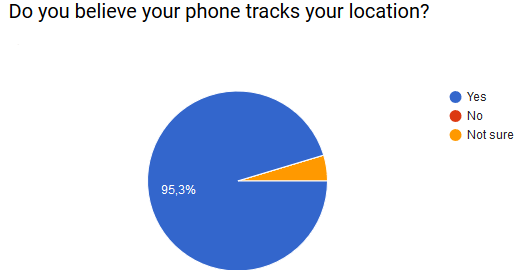
\includegraphics[width=0.8\textwidth]{survey/survey1}
  \caption{Survey question: location tracking}
  \label{fig:survey_location_tracking}
\end{figure}

This section of the survey focuses on the knowledge and awareness that the participant has about location tracking. The first question (see figure \ref{fig:survey_location_tracking}) asks whether the participant believes that his or her phone is tracking the phone's location. This was overwhelmingly answered with "Yes". Nobody has answered "No", and only two participants weren't sure. This goes to show that everyone is very aware of this kind of behaviour nowadays, which is most likely caused by the many privacy scandals of the past years, not only related to location tracking.

Going more into detail, fewer people know actual details on this subject. To the question \textit{"Do you believe that this location data is accessible to you as a user?"}, only 75\% think that the data is indeed accessible (speaking of Google Maps). Furthermore, only 37\% have ever seen the location history that Google has recorded of them. This 37\% mostly viewed their location history on the Google Maps website or mobile application (coming from a text answer field).

\subsection{Cartographer}

The last section now focuses on the application that we built within this project. We wanted to know if people are at all willing to use such an application and if they do, what features they would like the application to have.

Only every third participant was not interested in such an application, meaning that 67\% (29 out of 43 participants) were interested. Those people that were not interested received one more final question which was aimed to ask for the reason. Half of those participants answered that they had privacy concerns and the other half simply did not care enough about the subject.

Going further, we asked how comfortable the participant is with sharing their full location history with the application and therefore an unknown third-party provider. The results on this were very mixed, with a few people completely mistrusting the application, and a lot of people somewhere in the middle ranks (see figure \ref{fig:survey_location_access}).

\begin{figure}[ht]
    \center
    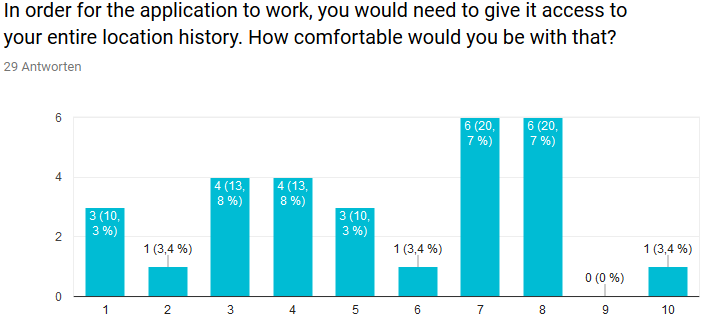
\includegraphics[width=1\textwidth]{survey/survey2}
    \caption{Survey: Access to the location history}
    \label{fig:survey_location_access}
\end{figure}

When asking for the desired functionality of the application, 97\% (everyone except one) of participants want to see their most frequent routes. 62\% want to have an overview of their most visited places, and 51\% want to have heat maps of their overall location history. Furthermore, 86\% want to get advice on how to improve their routes, and 69\% would like to get additional information about their most frequently visited places.

\subsection{Conclusion}

The answers to the questionnaire paint a clear picture that most people are aware of data collection practices by major companies such as Google. However, many people don't know much more than the fact that they're being "watched". The survey shows that many participants haven't even seen the data that is being collected on them, or is aware that they are able to see it.

This lack of awareness helps greatly with the demand of our application, because many are curious, what data is actually being collected on them. However, the survey also shows that many participants have concerns about the application's privacy practices and are unsure about it's trustworthiness. Because of this, it is important for us to be transparent and honest about our privacy policy and data handling.

The full survey with all questions and answers can be seen in Appendix \ref{FullSurvey}.

%----------------------------------------------------------------------------------------
%	FUTURE
%----------------------------------------------------------------------------------------

\newpage
\section{Future} \label{sec:Future}

Explain the future of this project and how the technology might evolve

%----------------------------------------------------------------------------------------
%	CONCLUSION
%----------------------------------------------------------------------------------------
\newpage
\section{Conclusion} \label{sec:Conclusion}

\textit{What information can you extract from the data that Google is collecting from you, specifically the location history?  How can we use that data for the user’s benefit?  Would users be interested in getting useful advice collected from that data?}

Google constantly track Android devices and store its information. When talking specifically about “Location History”, Google stores this information trying to be as accurate as possible.

Based on variables such as altitude, latitude, speed and heading (among others), Google tracks the activity the user is performing, choosing between the few most likely to be happening and sorting them by accuracy, giving a very reliable result.
By performing the same activity regularly, Google is able to guess workplaces, routines, home places, and so on.

All this information can be extracted from Google, available for every user for personal use, meaning each user can only access their own data. Also, this data can be edited and deleted by the user manually. 
The data containing the Location History can be extracted as a JSON file for simple reading or as a KML file, both with the full extension of its record (with no encryption whatsoever, leaving the file naked to the eye and lifting security questions). However, many users don't know how to access this information or if it even exists for personal use, as the survey results show.

We stress that the application works just as a vessel for the information stored by Google to be passed to the user in a visual form.
The user should be able to be aware of this information while the application process it and analyse the data, and provide the user with a better overview and understanding of it, with the mere objective of throwing some light over the data and let the user benefit from the knowledge acquired while using the application.

Although this data is not one hundred percent accurate since it is based on educated guesses, as pointed out before, it is very reliable in most of the cases, with the only precondition for the data to not be manipulated, in this case, the data would be considered corrupted and will lose credibility.

This data won’t be stored on any remote server, so the user will be the only responsible for the diffusion of its own information. Although, the application will inform the user about where the information will be stored, it will also ask the user to delete permanently any other file containing this information for security reasons, since the kind of databases this application uses is “hidden” (only if the device haven’t been rooted) and will be encrypted.

%----------------------------------------------------------------------------------------
%	BIBLIOGRAPHY
%----------------------------------------------------------------------------------------

\newpage
\printbibliography[heading=bibintoc,title={References}]

%----------------------------------------------------------------------------------------
%	APPENDIX
%----------------------------------------------------------------------------------------

\newpage
\appendix

\section{Appendix}

\subsection{Survey} \label{FullSurvey}

The following questions and answers show the full survey in text form.

\begin{enumerate}
    \item Are you an Android user?
    \begin{itemize}
        \item Yes (25 answers, 53,2\%)
        \item No (22 answers, 46,8\%)
    \end{itemize}
    
    \item Do you have the Google Maps application installed on your phone?
    \\\textit{Only displayed if answer was "No" in previous question.}
    \\\textit{Answering "No" ends the survey.}
    \begin{itemize}
        \item Yes (21 answers, 84\%)
        \item No (4 answers, 16\%)
    \end{itemize}
    
    \item Do you believe your phone tracks your location?
    \begin{itemize}
        \item Yes (41 answers, 95,3\%)
        \item No (0 answers, 0\%)
        \item Not sure (2 answers, 4,7\%)
    \end{itemize}
    
    \item Do you believe that this location data is accessible to you as a user?
    \begin{itemize}
        \item Yes (32 answers, 74,4\%)
        \item No (11 answers, 25,6\%)
    \end{itemize}
    
    \item Have you ever seen the location history that Google has recorded on you?
    \begin{itemize}
        \item Yes (16 answers, 37,2\%)
        \item No (27 answers, 62,8\%)
    \end{itemize}
    
    \item If yes, how did you gain access and in what format did you view it?
    \begin{itemize}
        \item Google Maps web \& mobile app
        \item Third party services
        \item Viewed it on my laptop, google maps
        \item Google send a message
        \item Google Maps mobile + desktop 
        \item Google maps shows me where i've been and when, but when i turn it off, i use a GPS mocker, and just place it at home. google maps thinks i'm home, snapchat thinks i'm home so privacy (even tho it's kinda a walk around)
        \item Google Maps
        \item computer
        \item Google Maps, Google+
        \item Google Maps mobile app
        \item Laptop
        \item Google Maps Timeline (mobile, desktop), Google Fit (mobile), Google Search and Search History (mobile), Google Settings (desktop when logged in) + several mobile apps that implement a location feature
        \item I used Google Timeline and Takeout
    \end{itemize}
    
    \item Would you be willing to use an application that can present you an in-depth analysis of your location history?
    \begin{itemize}
        \item Yes (29 answers, 67,4\%)
        \item No (14 answers, 32,6\%)
    \end{itemize}
    
    \item Why not?
    \\\textit{This question is only displayed if the previous answer was "No". The survey ends after this question.}
    \begin{itemize}
        \item Privacy concerns (7 answers, 50\%)
        \item I don't care (6 answers, 42,9\%)
        \item I don't care since it wont affect Google tracking my location either way. If it blocked the data gathering from google then yes. (1 answer, 7,1\%)
    \end{itemize}
    
    \item In order for the application to work, you would need to give it access to your entire location history. How comfortable would you be with that?
    \\\textit{The answers are on a scale from 1 to 10, with 10 being the most comfortable.}
    \begin{itemize}
        \item 10 (1 answer, 3,4\%)
        \item 9 (0 answers, 0\%)
        \item 8 (6 answers, 20,7\%)
        \item 7 (6 answers, 20,7\%)
        \item 6 (1 answer, 3,4\%)
        \item 5 (3 answers, 10,3\%)
        \item 4 (4 answers, 13,8\%)
        \item 3 (4 answers, 13,8\%)
        \item 2 (1 answer, 3,4\%)
        \item 1 (3 answers, 10,3\%)
    \end{itemize}

    \item What functionality would you like the app to have?
    \\\textit{This is a multiple choice question. The percentage shows how many participants want a certain feature.}
    \begin{itemize}
        \item Heat maps (15 answers, 51,7\%)
        \item Most visited places (18 answers, 62,1\%)
        \item Most frequent routes (28 answers, 96,6\%)
    \end{itemize}
    
    \item Would you like to get advice on how to improve your commute?
    \begin{itemize}
        \item Yes (25 answers, 86,2\%)
        \item No (4 answers, 13,8\%)
    \end{itemize}
    
    \item Would you like to get additional information about your most frequently visited places?
    \begin{itemize}
        \item Yes (20 answers, 69\%)
        \item No (9 answers, 31\%)
    \end{itemize}
\end{enumerate}

%------------------------------------------------
		
\end{document}